\documentclass[10pt,mathserif]{beamer}

\input defs.tex

%\setbeamerfont*{frametitle}{size=\normalsize,series=\bfseries}

% from boyd
\mode<presentation>
{
\usetheme{default}
}
\setbeamertemplate{navigation symbols}{}
\usecolortheme[rgb={0.13,0.28,0.59}]{structure}
\setbeamertemplate{itemize subitem}{--}
\setbeamertemplate{frametitle} {
	\begin{center}
	  {\large\bf \insertframetitle}
	\end{center}
}

\newcommand\footlineon{
  \setbeamertemplate{footline} {
    \begin{beamercolorbox}[ht=2.5ex,dp=1.125ex,leftskip=.8cm,rightskip=.6cm]{structure}
      \footnotesize \insertsection
      \hfill
      {\insertframenumber}
    \end{beamercolorbox}
    \vskip 0.45cm
  }
}
\footlineon

\newcommand\blfootnote[1]{%
  \begingroup
  \renewcommand\thefootnote{}\footnote{#1}%
  \addtocounter{footnote}{-1}%
  \endgroup
}

\AtBeginSection[] 
{ 
\begin{frame}<beamer> 
\frametitle{Outline} 
\tableofcontents[currentsection] 
\end{frame} 
}


%
\usepackage{alphalph}
\usepackage{array}
\usepackage{graphics}
\usepackage{animate}
\usepackage[export]{adjustbox}
\usepackage{centernot}
\usepackage{caption}
\usepackage{subcaption}
\usepackage{booktabs} % for professional tables
\usepackage{multirow}
\usepackage{microtype}
\usepackage{graphicx}
\usepackage{amsmath, amssymb, amsthm}
\usepackage{dsfont}
\usepackage{mathtools}
\usepackage{algorithm,algorithmic}
\usepackage{adjustbox}
% Setup TikZ
\usepackage{tikz}
\usepackage{tkz-graph}
\usepackage{pgfplots}
\usepackage{hyperref}

\usepackage[beamer]{hf-tikz} 
\usetikzlibrary{backgrounds,arrows,shapes.geometric,shapes.misc,positioning,patterns}


\tikzstyle{block}=[draw opacity=0.7,line width=1.4cm]

\newcommand{\norm}[1]{\left\lVert#1\right\rVert}

\renewcommand{\algorithmicrequire}{\textbf{initialize}}
\newcommand{\algorithmicinput}{\textbf{input}}
\newcommand{\algorithmicoutput}{\textbf{output}}
\newcommand{\INPUT}{\item[\algorithmicinput]}
\newcommand{\OUTPUT}{\item[\algorithmicoutput]}

\setbeamertemplate{theorems}[numbered]
\newtheorem{thm}{Theorem}
\newtheorem{defn}{Definition}
\newtheorem{prop}{Proposition}

% Author, Title, etc.
\title{Machine Learning Research at SNU Machine Learning Lab}
\author{Hyun Oh Song}
\institute
    {Seoul National University}
\date{2019.04.19}

% hide solutions in handout mode
\newcommand\hideit[1]{%
  \only<0| handout:1>{\mbox{}}%
  \invisible<0| handout:1>{#1}}

% independence symbol
\newcommand{\indep}{\raisebox{0.05em}{\rotatebox[origin=c]{90}{$\models$}}}
\tikzset{above left offset={0.0,0.6},below right offset={0.0,-0.5}}

% The main document
\begin{document}
\begin{frame}
  \titlepage
\end{frame}

\section{EMI: Exploration with Mutual Information}
%%\subsection{Background} % Sections can be created in order to organize your presentation into discrete blocks, all sections and subsections are automatically printed in the table of contents as an overview of the talk
%------------------------------------------------
%%\subsection{Intro}
\setbeamercolor{block body}{parent=normal text,use=block title,bg=block title.bg!15!bg}
\setbeamercolor{block title}{use=structure,fg=white,bg=structure.fg!75!black}


\begin{frame}
\frametitle{Reinforcement Learning}
  \textbf{Reinforcement Learning} is learning by interacting with environments.

  \begin{itemize} \itemsep=6pt
      \item Learn from consequences of actions.
      \item Receives reinforcement signal (reward).
      \item Seeks to maximize accumulated reward.
  \end{itemize}
  \begin{figure}[h]
        \centering
          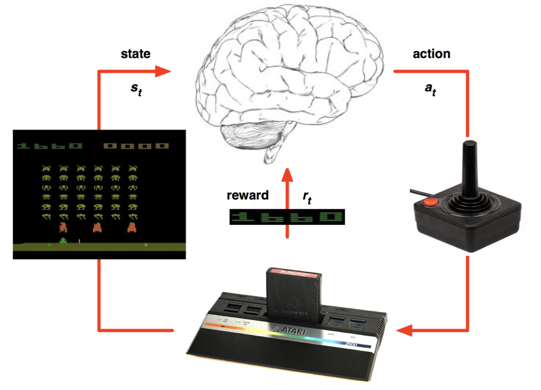
\includegraphics[width=0.7\textwidth]{emi_figures/mk_intro}
  \end{figure}
\end{frame}

%------------------------------------------------

\begin{frame}
\frametitle{Reinforcement learning objective}

	Let $\pi$ denote a stochastic policy $\pi : S \times A \rightarrow [0, 1]$, and let $\eta(\pi)$ denote its expected discounted reward:
	\begin{align*}
	&\eta(\pi) = \mathbb{E}_{s_0, a_0, \cdots} \left[ \sum_{t=0}^{\infty} \gamma^t r(s_t) \right], \text{where} \\
	&\quad s_0 \sim \rho_0(s_0), a_t \sim \pi(a_t | s_t), s_{t+1} \sim P(s_{t+1} | s_t, a_t).
	\end{align*}
  \begin{figure}[h]
        \centering
          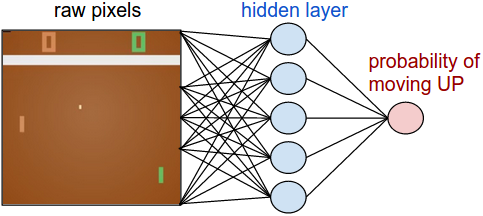
\includegraphics[width=0.7\textwidth]{emi_figures/pg_policy}
          \caption{Example policy network of Atari 2600 Pong.}
  \end{figure}
\end{frame}

%------------------------------------------------

\begin{frame}
\frametitle{Sparse reward environments}
  \begin{itemize} \itemsep=6pt
      \item It is hard to learn policy in sparse reward environments.
      \item How can we explore sparse reward environments efficiently?
  \end{itemize}

  \begin{figure}[h]
        \centering
          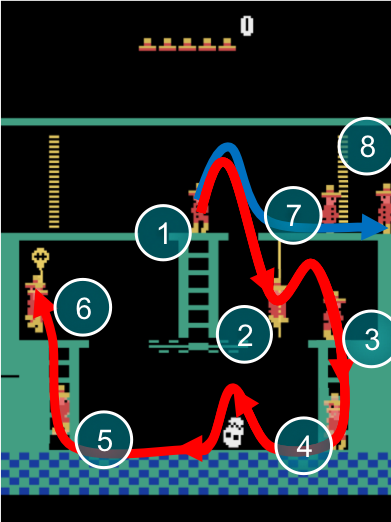
\includegraphics[width=0.3\textwidth]{emi_figures/bc_montezuma}
          \caption{Agent should move in $1 \rightarrow 2 \rightarrow 3 \rightarrow 4 \rightarrow 5 \rightarrow 6$ to get the reward signal.}
  \end{figure}
\end{frame}

%------------------------------------------------

%%\subsection{Methods} % Sections can be created in order to organize your presentation into discrete blocks, all sections and subsections are automatically printed in the table of contents as an overview of the talk

%------------------------------------------------

\begin{frame}
\frametitle{Intuition}
  \begin{itemize} \itemsep=6pt
      \item Construct \textbf{the embedding representations} of the observation and action.
      \item Measure \textbf{the novelty} of encountering states with embedding representations.
  \end{itemize}
  \pause

  \begin{figure}[h]
        \centering
          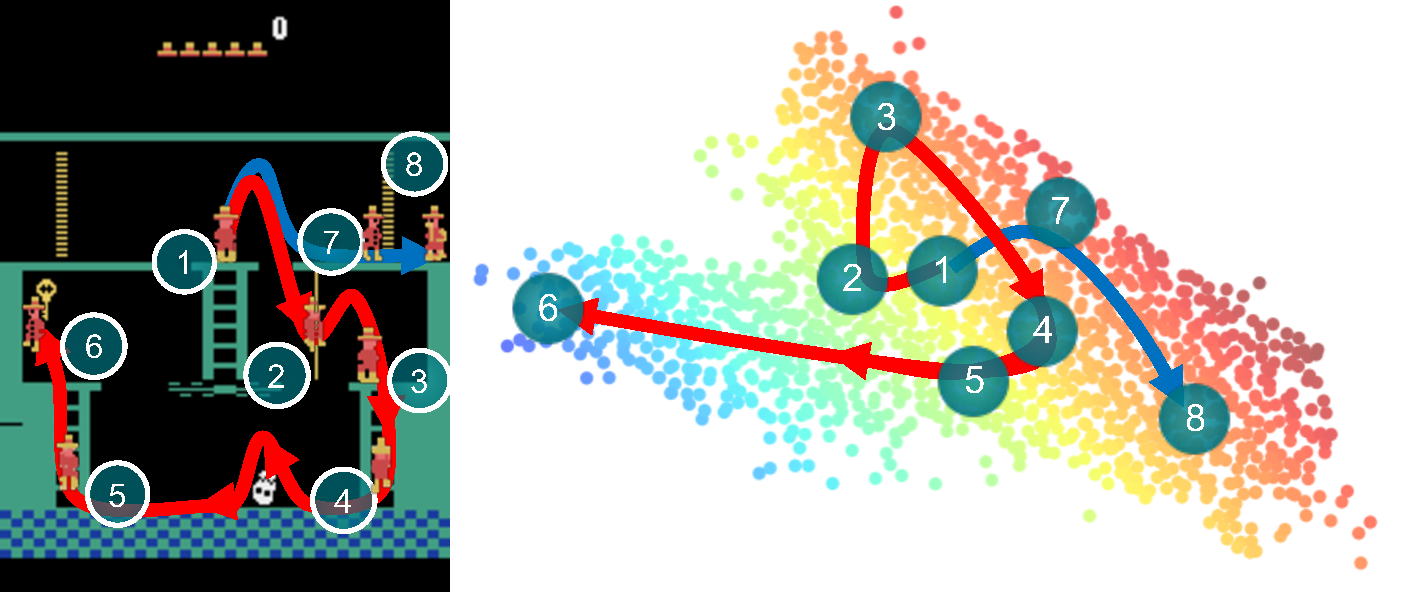
\includegraphics[width=0.7\textwidth]{emi_figures/figure_embedding_concept}
          \caption{Visualization of a sample trajectory in our learned embedding space.}
  \end{figure}

\end{frame}


%------------------------------------------------

\begin{frame}
\frametitle{Learn embedding representations}

Learn embedding of states $\phi_\alpha : \mathcal{S} \rightarrow \reals^d$ and actions $\psi_\beta: \mathcal{A} \rightarrow \reals^d$.
\vspace{1em}

\begin{enumerate} \itemsep=12pt
\item Given $[\phi_\alpha(s); \psi_\beta(a)]$, the uncertainty of the embedding representation of the corresponding next states $\phi_\alpha(s')$ should be minimal and vice versa. \pause

\item Given $[\phi_\alpha(s); \phi_\alpha(s')]$, the uncertainty of the embedding representation of the corresponding actions $\psi_\beta(a)$ should also be minimal and vice versa.

\end{enumerate}
\end{frame}

%------------------------------------------------

\begin{frame}
\frametitle{Learn embedding representations}

Learn embedding of states $\phi_\alpha : \mathcal{S} \rightarrow \reals^d$ and actions $\psi_\beta: \mathcal{A} \rightarrow \reals^d$.

\begin{align}
\text{1. }\maximize_{\alpha, \beta}~ \mathcal{I}_S(\alpha, \beta) &:= \mathcal{I}([\phi_\alpha(s); \psi_\beta(a)]; \phi_\alpha(s')) \nonumber \\
&= \mathcal{D}_{\text{KL}}\left(\mathbb{P}_{SAS'}^\pi \parallel \mathbb{P}_{SA}^\pi \otimes \mathbb{P}_{S'}^\pi\right) \nonumber
%\label{eqn:infogain_s}
\end{align}\pause
\vspace{-1em}
\begin{align}
\text{2. }\maximize_{\alpha, \beta}~ \mathcal{I}_A(\alpha, \beta) &:= \mathcal{I}([\phi_\alpha(s); \phi_\alpha(s')]; \psi_\beta(a)) \nonumber \\
&= \mathcal{D}_{\text{KL}}\left(\mathbb{P}_{SAS'}^\pi \parallel \mathbb{P}_{SS'}^\pi \otimes \mathbb{P}_A^\pi\right) \nonumber
%\label{eqn:infogain_a}
\end{align}

\end{frame}

%------------------------------------------------
\begin{frame}
\begin{thm}\label{thm:emi_js}
The lower bound of mutual information using Jensen-Shannon divergence:
\begin{align*}
    \mathcal{I}^{(\text{JSD})}(X; Z) &\geq \sup_{\omega \in \Omega} 
    \mathbb{E}_{\mathbb{P}_{XZ}} \left[-\text{sp} \left(-T_{\omega}(x,z)\right)\right] \\
    & - \mathbb{E}_{\mathbb{P}_{X} \otimes \mathbb{P}_Z} \left[ \text{sp} \left(T_{\omega}(x,z)\right)\right]+\log(4)
\end{align*}
\end{thm}
\end{frame}

%------------------------------------------------

\begin{frame}
\begin{proof}
\begin{align*}
    &\mathcal{I}^{(\text{JSD})}(X; Z) = \mathcal{D}_\text{JSD}(\mathbb{P}_{XZ} \parallel \mathbb{P}_{X} \otimes \mathbb{P}_Z)\nonumber\\
    &\geq \sup_{\omega \in \Omega} \mathbb{E}_{\mathbb{P}_{XZ}} \left[S_\omega(x,z)\right] - \mathbb{E}_{\mathbb{P}_{X} \otimes \mathbb{P}_Z} \left[\text{JSD}^{*}\left(S_\omega(x,z)\right)\right] \nonumber\\
    &= \sup_{\omega \in \Omega} \mathbb{E}_{\mathbb{P}_{XZ}} \left[-\text{sp} \left(-T_{\omega}(x,z)\right)\right] \nonumber \\ 
    & \qquad \quad - \mathbb{E}_{\mathbb{P}_{X} \otimes \mathbb{P}_Z} \left[ \text{sp} \left(T_{\omega}(x,z)\right)\right] +\log(4),
\end{align*}
where the inequality in the second line holds from the definition of $f$-divergence. In the third line, we substituted $S_\omega(x,z) = \log(2) - \log(1+\exp(-T_\omega(x,z)))$ and \textit{Fenchel conjugate} of Jensen-Shannon divergence, $\text{JSD}^{*}(t) = -\log(2-\exp(t))$.
\end{proof}
\end{frame}

%------------------------------------------------

\begin{frame}
\frametitle{Learn embedding representations}

Learn embedding of states $\phi_\alpha : \mathcal{S} \rightarrow \reals^d$ and actions $\psi_\beta: \mathcal{A} \rightarrow \reals^d$.


\begin{align} 
%\label{eqn:infogain_s_jsd}
\text{1. }\maximize_{\alpha, \beta}&~ \mathcal{I}^{\text{(JSD)}}_S(\alpha, \beta) \nonumber \\
\geq& \maximize_{\alpha, \beta}  \sup_{\omega_S \in \Omega_S}\mathbb{E}_{\mathbb{P}_{SAS'}^\pi} \left[-\text{sp} \left(-T_{\omega_S}(\phi_\alpha(s), \psi_\beta(a), \phi_\alpha(s'))\right)\right] \nonumber \\
& -\mathbb{E}_{\mathbb{P}_{SA}^\pi \otimes \mathbb{P}_{S'}^\pi} \left[ \text{sp} \left(T_{\omega_S}(\phi_\alpha(s), \psi_\beta(a), \phi_\alpha(\tilde{s'}))\right)\right] + \log{4} \nonumber
\end{align}\pause
\begin{align}
%\label{eqn:infogain_a_jsd}
\text{2. }\maximize_{\alpha, \beta}&~ \mathcal{I}^{\text{(JSD)}}_A(\alpha, \beta) \nonumber \\
\geq& \maximize_{\alpha, \beta}  \sup_{\omega_A \in \Omega_A} \mathbb{E}_{\mathbb{P}_{SAS'}^\pi} \left[-\text{sp} \left(-T_{\omega_A}(\phi_\alpha(s), \psi_\beta(a), \phi_\alpha(s'))\right)\right] \nonumber \\
& -\mathbb{E}_{\mathbb{P}_{SS'}^\pi \otimes \mathbb{P}_{A}^\pi} \left[ \text{sp} \left(T_{\omega_A}(\phi_\alpha(s), \psi_\beta(\tilde{a}), \phi_\alpha(s'))\right)\right] +\log{4} \nonumber
\end{align}

\end{frame}

%------------------------------------------------

\begin{frame}
\frametitle{Architecture of EMI}
  \vspace{2em}
  \hspace*{-2em} 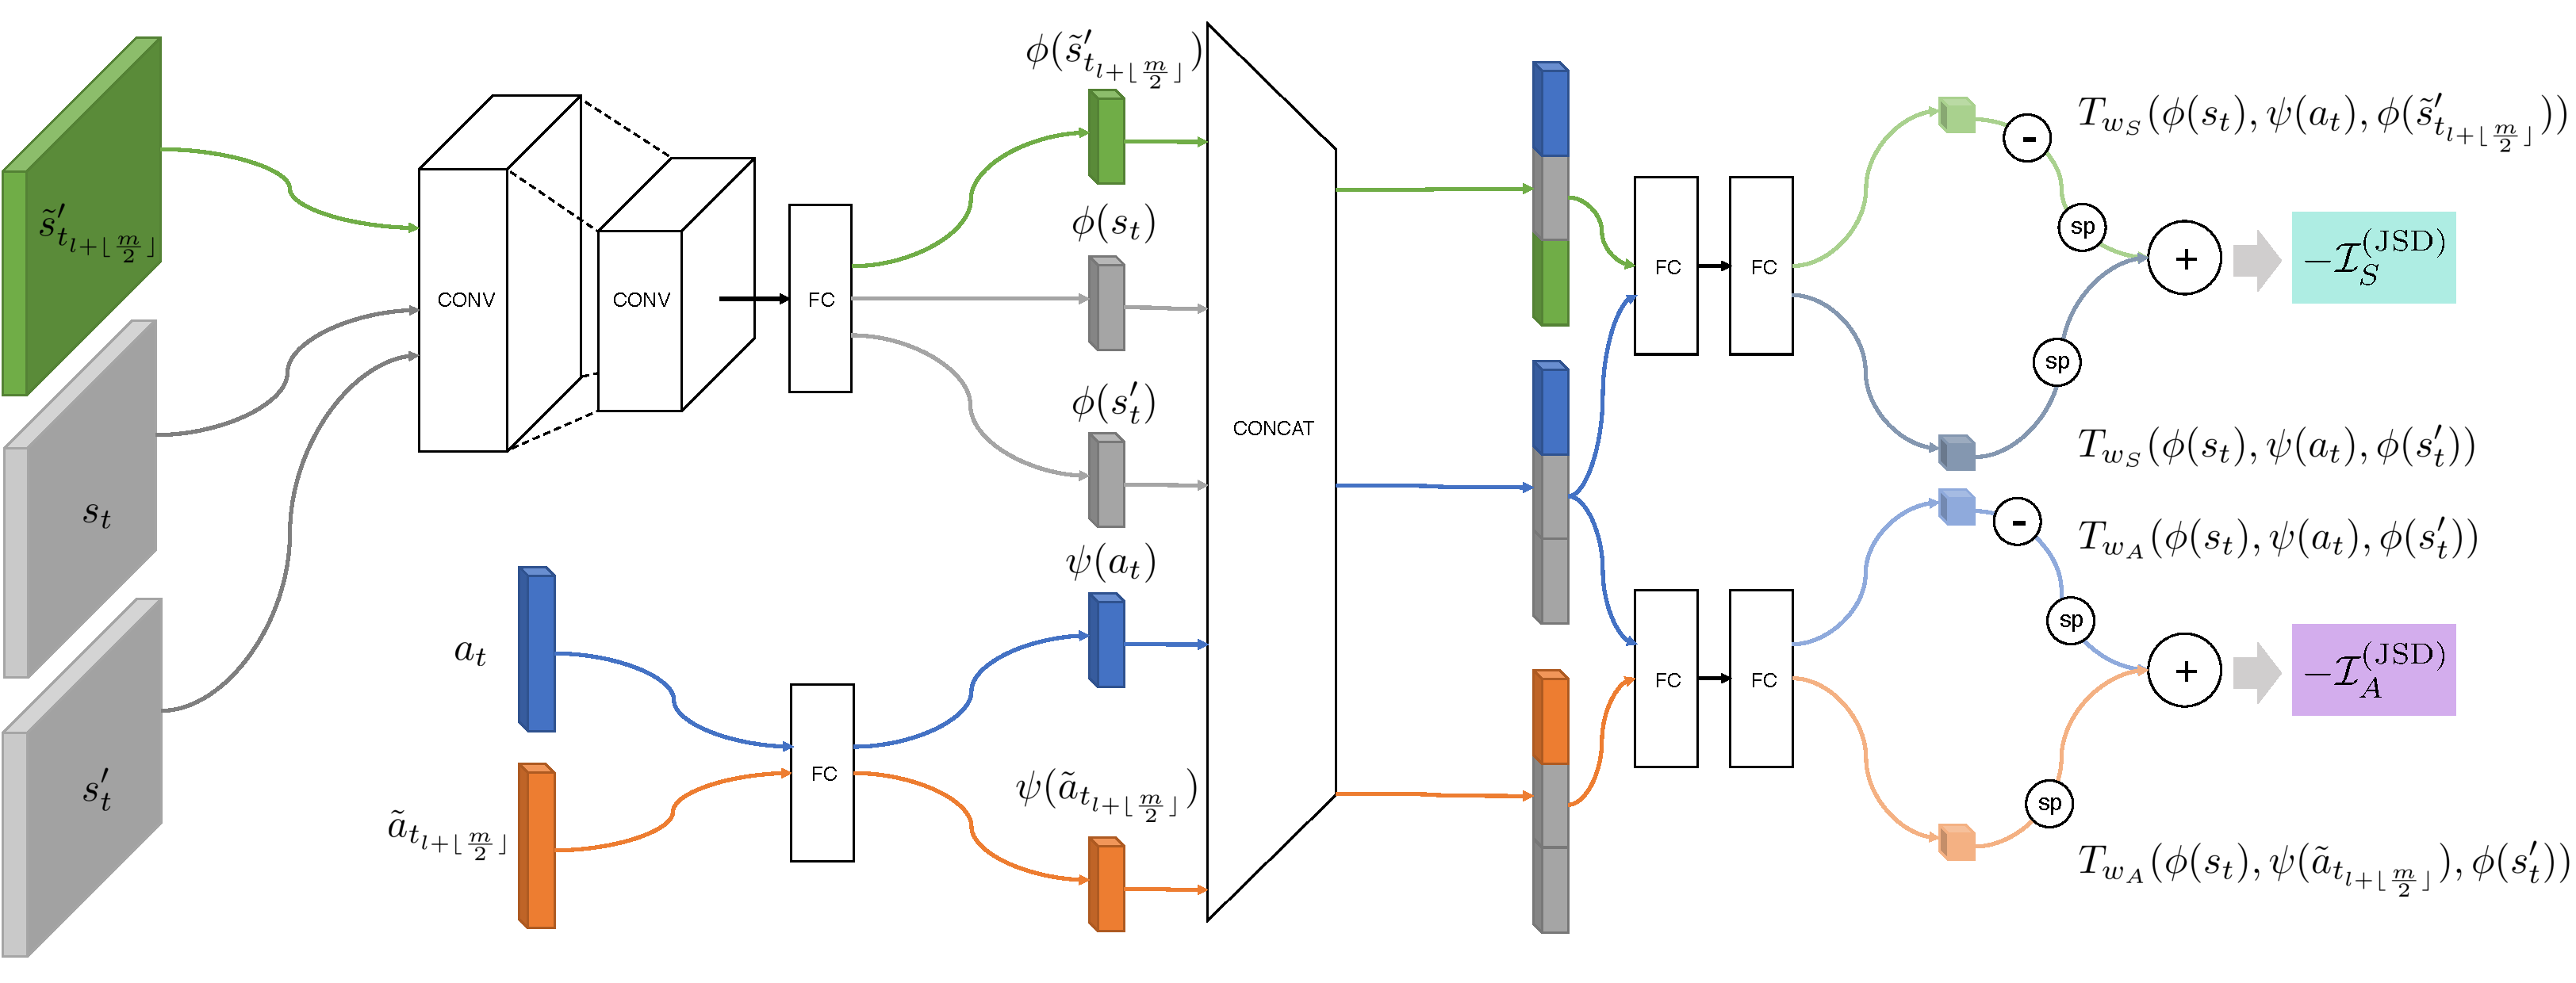
\includegraphics[width=0.95\paperwidth]{emi_figures/arch_diagram}
  \vspace{-1em}
  \begin{figure}
      \caption{Computational architecture for estimating $\mathcal{I}^{\text{(JSD)}}_S$ and $\mathcal{I}^{\text{(JSD)}}_A$ for image-based observations.}
  \end{figure}

\end{frame}

%------------------------------------------------

\begin{frame}
\frametitle{Linear dynamics model with error model}
\begin{itemize} \itemsep=12pt
\item Learn $\phi(s)$ and $\psi(a)$ such that $\phi(s')$ follow linear dynamics \ie~ $\phi(s') = \phi(s) + \psi(a)$.
\item Offload irreducible error to the error model $S_\gamma : \mathcal{S} \times \mathcal{A} \rightarrow \reals^d$.
\end{itemize}

\begin{align}
&\minimize_{\alpha, \beta, \gamma} \underbrace{\| S_\gamma \|_{2,0}}_{\text{error minimization}} \nonumber\\
&\text{\ subject to }~~ \underbrace{\Phi_{\alpha}' = \Phi_\alpha + \Psi_\beta + S_\gamma}_{\text{embedding linear dynamics}}, \nonumber
%\label{eqn:sparse}
\end{align}

\end{frame}

%------------------------------------------------

\begin{frame}
\frametitle{Learning objective}

\begin{align} 
\minimize_{\alpha, \beta, \gamma} ~ &\|\Phi'_\alpha - \left( \Phi_\alpha + \Psi_\beta  + S_\gamma \right)\|_F^2 \nonumber\\
&+ \lambda_{\text{error}} \| S_\gamma \|_F^2
+ \lambda_\text{info} \mathcal{L}_\text{info}, \nonumber
\end{align}
%\vspace{-5em}
\begin{align}
\text{where, }\mathcal{L}_\text{info} &= \inf_{\omega_S \in \Omega_S} \mathbb{E}_{\mathbb{P}_{SAS'}^\pi} \text{sp} \left(-T_{\omega_S}(\phi_\alpha(s), \psi_\beta(a), \phi_\alpha(s'))\right) \nonumber \\
&\qquad \quad + \mathbb{E}_{\mathbb{P}_{SA}^\pi \otimes \mathbb{P}_{S'}^\pi} ~\text{sp} \left(T_{\omega_S}(\phi_\alpha(s), \psi_\beta(a), \phi_\alpha(\tilde{s'}))\right) \nonumber \\
&+ \inf_{\omega_A \in \Omega_A} \mathbb{E}_{\mathbb{P}_{SAS'}^\pi} \text{sp} \left(-T_{\omega_A}(\phi_\alpha(s), \psi_\beta(a), \phi_\alpha(s'))\right) \nonumber \\
&\qquad \quad + \mathbb{E}_{\mathbb{P}_{SS'}^\pi \otimes \mathbb{P}_{A}^\pi} ~\text{sp} \left(T_{\omega_A}(\phi_\alpha(s), \psi_\beta(\tilde{a}), \phi_\alpha(s'))\right) \nonumber
\end{align}


\end{frame}
%------------------------------------------------

\begin{frame}
\frametitle{Intrinsic reward augmentation}
Measure the novelty with prediction error under the linear dynamics model and use it as intrinsic reward.
\begin{align}
\hspace{-0.5em}  r_i(s_t, a_t, s_t') = \|\phi(s_t) + \psi(a_t) + S(s_t, a_t) - \phi(s_t')\|^2 \nonumber
%\label{eqn:ir_err}
\end{align}
\end{frame}

%------------------------------------------------

\begin{frame}
\frametitle{Pseudocode}
  \begin{figure}[h]
        \centering
          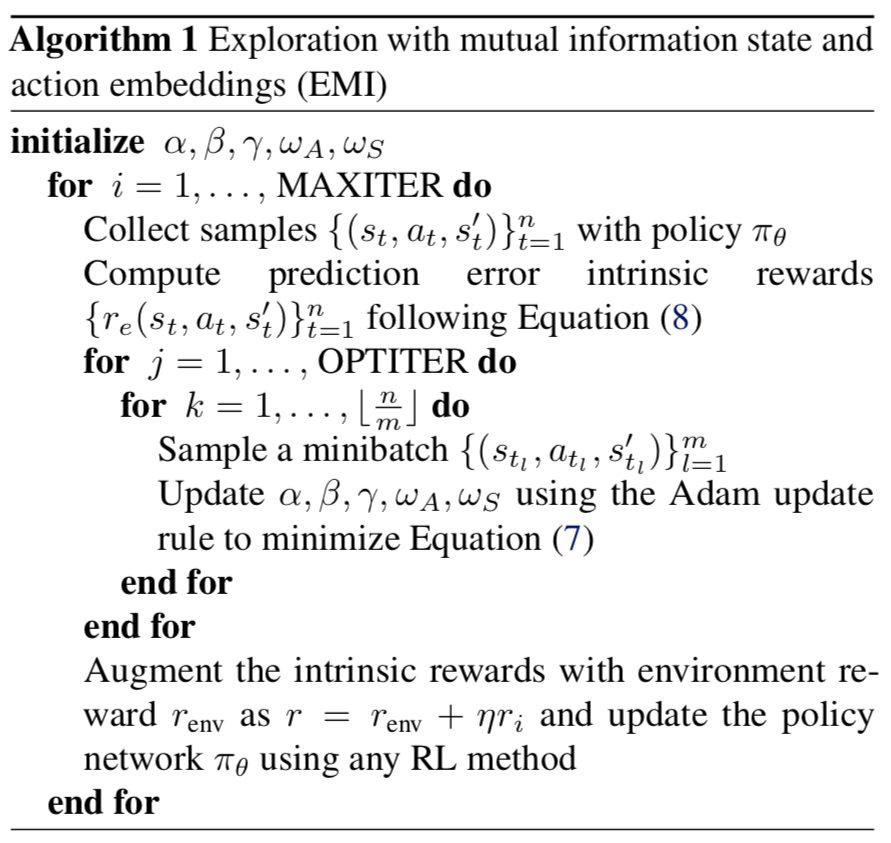
\includegraphics[width=0.7\textwidth]{emi_figures/emi_alg}
  \end{figure}
\end{frame}

%------------------------------------------------

%%\subsection{Experiments} % Sections can be created in order to organize your presentation into discrete blocks, all sections and subsections are automatically printed in the table of contents as an overview of the talk

%------------------------------------------------

\begin{frame}
\frametitle{Baselines}
  \begin{itemize} \itemsep=12pt
    \item We compare EMI with five exploration baselines on top of TRPO\footnote{{\color{blue} J. Schulman, S. Levine, P. Abbeel, M. Jordan, and P. Moritz.} ``Trust region policy optimization''. \textcolor{gray}{ICML2015.}}.
    \uncover<2->{\item EX2\footnote<2->{{\color{blue} J. Fu, J. Co-Reyes, and S. Levine.} ``Ex2: Exploration with exemplar models for deep reinforcement learning''. \textcolor{gray}{NIPS2017.}} trains an ensemble model to estimate state visitation densities, and leads the agent to rarely visited states.}
    \uncover<3->{\item ICM\footnote<3->{{\color{blue} D. Pathak, P. Agrawal, A. Efros, and T. Darrell.} ``Curiosity-driven exploration by self-supervised prediction''. \textcolor{gray}{ICML2017.}} forms forward and inverse dynamics models and uses prediction errors as exploration signals.}
  \end{itemize}

\end{frame}

%------------------------------------------------

\begin{frame}
\frametitle{Baselines}
  \begin{itemize} \itemsep=12pt
    \item RND\footnote{{\color{blue} Y. Burda, H. Edwards, A. Storkey, and O. Klimov.} ``Exploration by random network distillation''. \textcolor{gray}{ICLR2019.}} trains a network to predict the output of a fixed randomly initialized network and employs the prediction errors for exploration.
    \renewcommand*{\thefootnote}{\fnsymbol{footnote}}\footnotetext<2->{\label{noteFinalPerformanceOnly}For final performance comparison only.}\renewcommand*{\thefootnote}{\arabic{footnote}}
    \uncover<2->{\item AE-SimHash\footnote<2->{{\color{blue} H. Tang, R. Houthooft, D. Foote, A. Stooke, X. Chen, Y. Duan,  J. Schulman, F. De Turck, and P. Abbeel.} ``\# Exploration: A study of count-based exploration for deep reinforcement learning''. \textcolor{gray}{NIPS2017.}}\textsuperscript{\ref{noteFinalPerformanceOnly}} computes hash codes for input states by training an autoencoder, and generates count-based exploration signals with the hash codes.}
    \uncover<3->{\item VIME\footnote<3->{{\color{blue} R. Houthooft, X. Chen, Y. Duan, J. Schulman, F. De Turck, and P. Abbeel.} ``Vime: Variational information maximizing exploration''. \textcolor{gray}{NIPS2016.}}\textsuperscript{\ref{noteFinalPerformanceOnly}} approximates the environment dynamics and uses the information gain of the learned dynamics model as intrinsic rewards.}
  \end{itemize}
\end{frame}

%------------------------------------------------
\begin{frame}
\frametitle{Environments}
  \begin{itemize} \itemsep=6pt
    \item Use sparse-reward environments to evaluate and compare the exploration capabilities of the baseline methods and EMI.
    \item \textit{SwimmerGather} and \textit{SparseHalfCheetah} from MuJoCo for locomotion tasks with continuous control.
    \item Six Atari environments, \textit{Freeway}, \textit{Frostbite}, \textit{Venture}, \textit{Montezuma's Revenge}, \textit{Gravitar}, and \textit{Solaris} from Arcade Learning Environment for vision-based tasks with discrete control.
  \end{itemize}
  \pause
  \vspace{1em}
  
  \begin{figure}[h]
    \centering
    \begin{subfigure}[t]{0.3\textwidth}
        \centering
        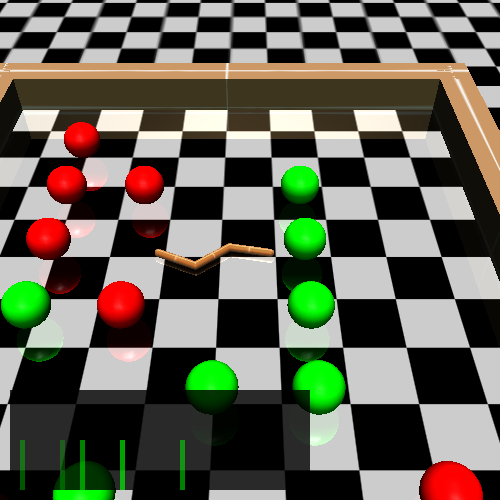
\includegraphics[height=7em,right]{emi_figures/env_image_SwimmerGather.png}
    \end{subfigure}
    \begin{subfigure}[t]{0.3\textwidth}
        \centering
        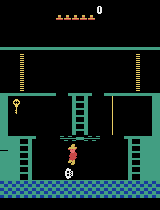
\includegraphics[height=7em,center]{emi_figures/env_image_MontezumaRevenge.png}
    \end{subfigure}
    \begin{subfigure}[t]{0.3\textwidth}
        \centering
        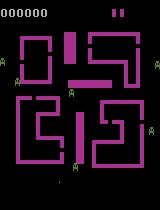
\includegraphics[height=7em,left]{emi_figures/env_image_Venture.png}
    \end{subfigure}
    \caption{Example scenes from \textit{SwimmerGather} (left), \textit{Montezuma's Revenge} (middle), and \textit{Venture} (right).}
  \end{figure}

\end{frame}

%------------------------------------------------

\begin{frame}
\frametitle{Comparison of average returns}
  \begin{figure}[ht!]
      \centering
      \begin{subfigure}{0.32\textwidth}
          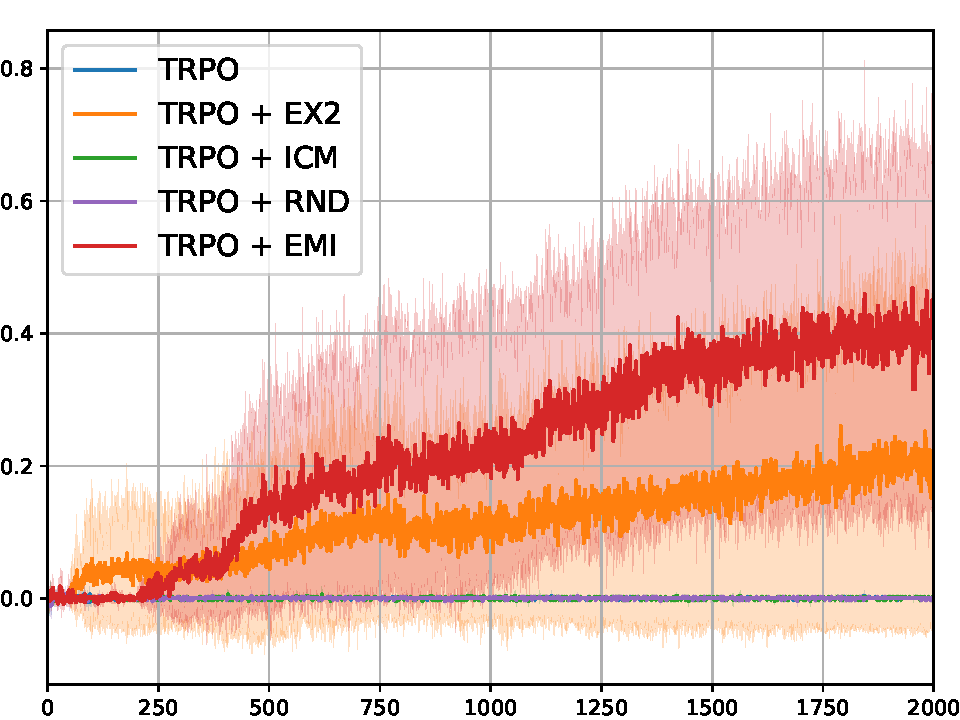
\includegraphics[width=\textwidth]{emi_figures/SwimmerGather_all.pdf}
          \caption{\textit{SwimmerGather}}
      \end{subfigure}
      \begin{subfigure}{0.32\textwidth}
          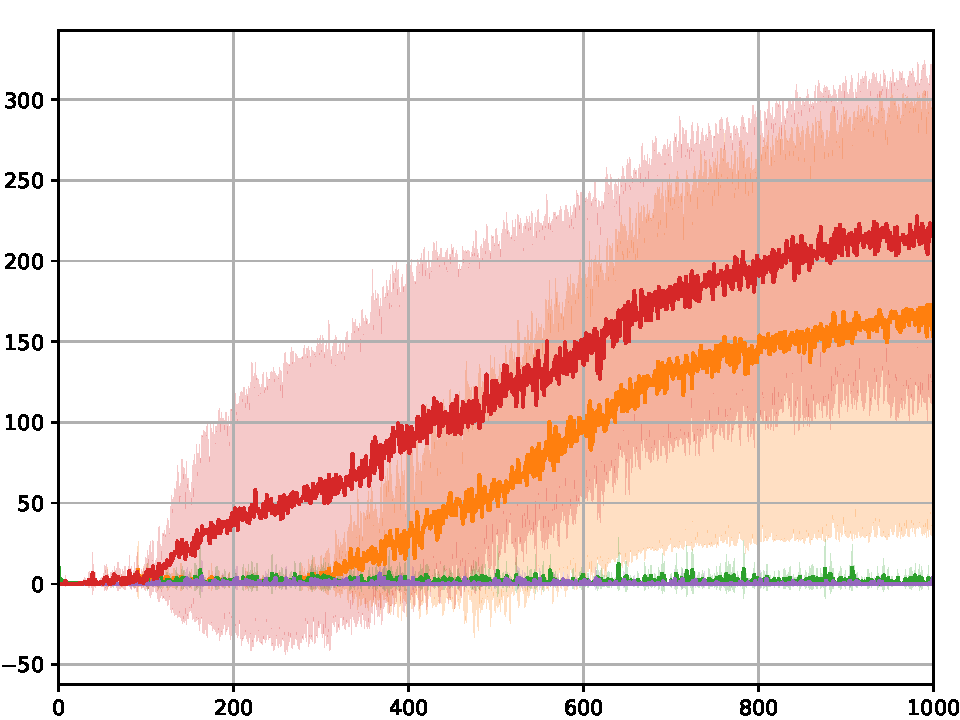
\includegraphics[width=\textwidth]{emi_figures/SparseHalfCheetah_all.pdf}
          \caption{\textit{SparseHalfCheetah}}
      \end{subfigure}
      \begin{subfigure}{0.32\textwidth}
          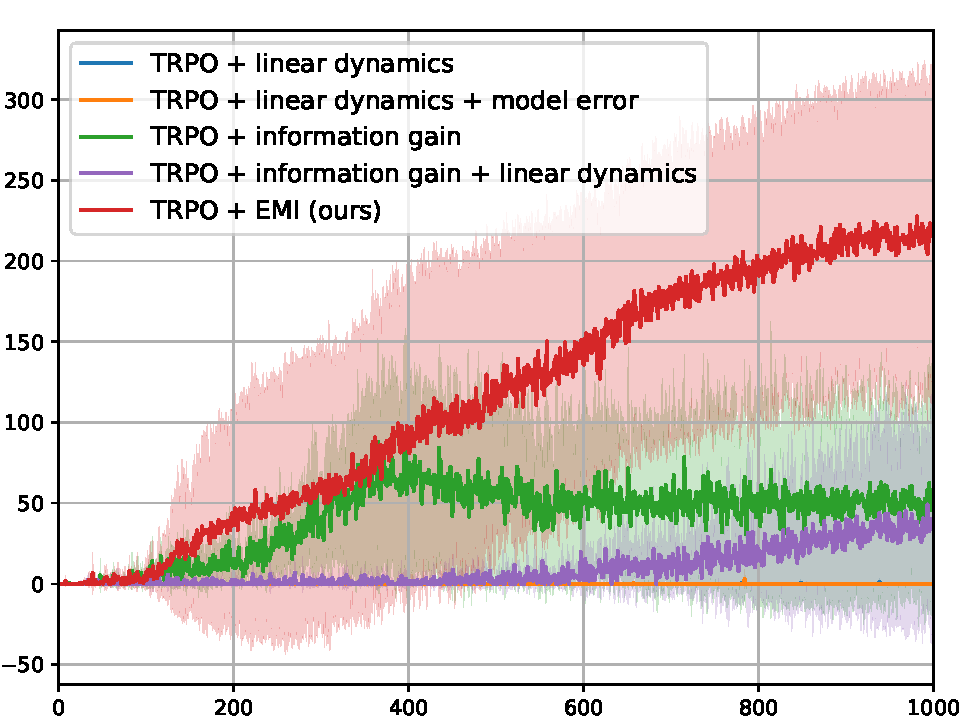
\includegraphics[width=\textwidth]{emi_figures/SparseHalfCheetah_ablate_loss.pdf}
   	      \caption{Ablation study}
      \end{subfigure}
      \caption{(a), (b): Performance of EMI on locomotion tasks with sparse rewards compared to baseline methods. The solid lines show the mean reward (y-axis) of 5 different seeds at each iteration (x-axis) and the shaded area represents one standard deviation from the mean. (c): Ablation result on \textit{SparseHalfCheetah}.}
  \end{figure}
\end{frame}


%------------------------------------------------

\begin{frame}
\frametitle{Comparison of average returns}
\begin{figure}[ht!]
  \resizebox{0.8\columnwidth}{!}{
    \centering
    \begin{subfigure}{0.32\textwidth}
        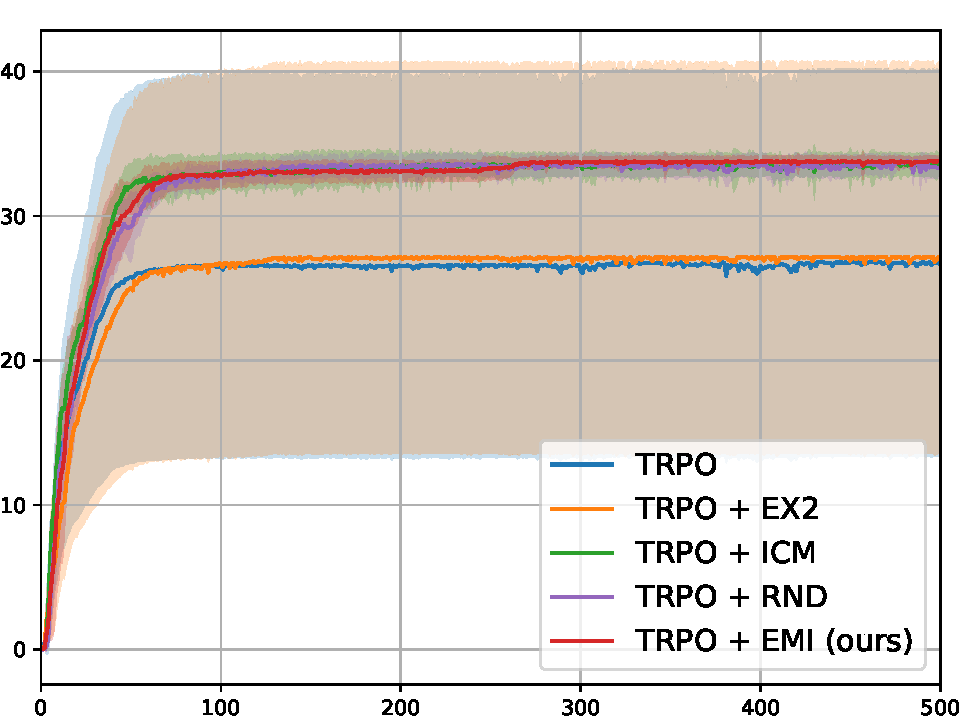
\includegraphics[width=\textwidth]{emi_figures/Freeway_all.pdf}
        \caption{\textit{Freeway}}
    \end{subfigure}
    \begin{subfigure}{0.32\textwidth}
        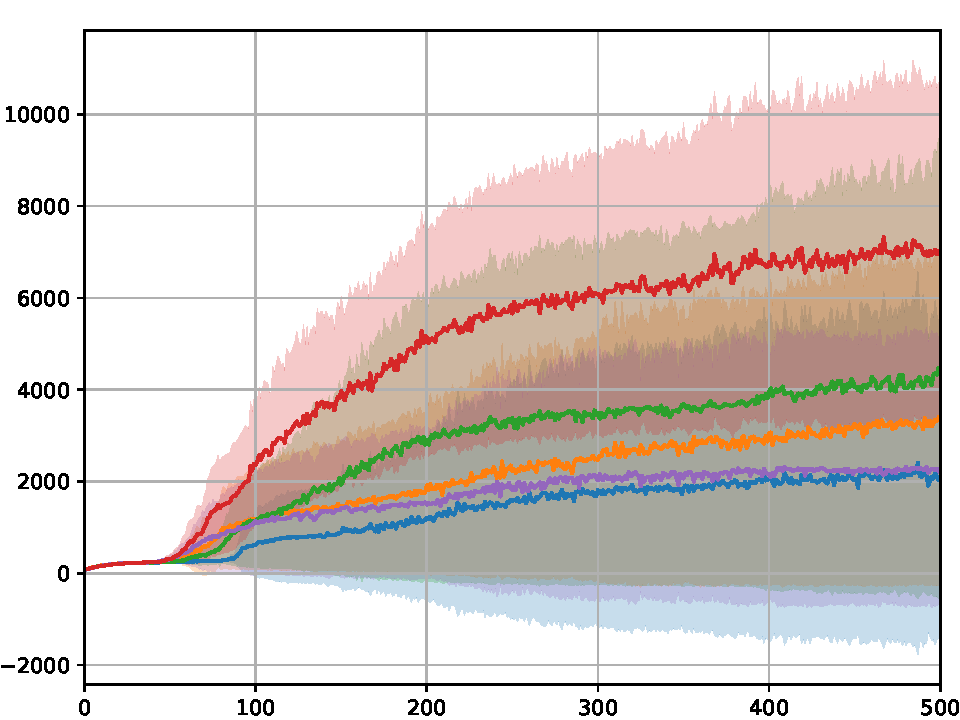
\includegraphics[width=\textwidth]{emi_figures/Frostbite_all.pdf}
        \caption{\textit{Frostbite}}
    \end{subfigure}
    \begin{subfigure}{0.32\textwidth}
        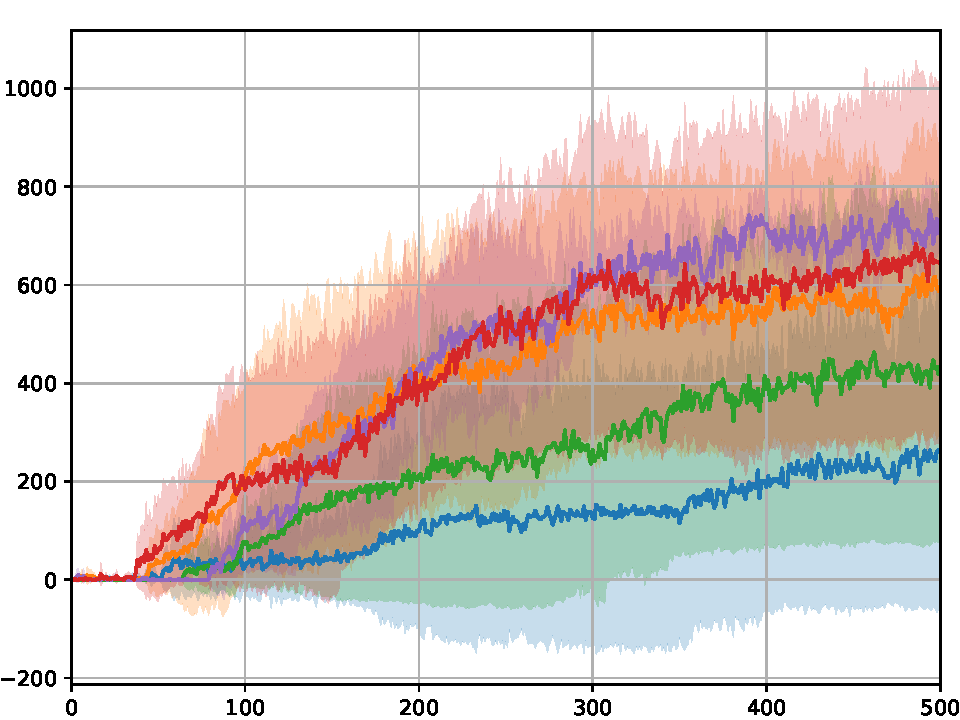
\includegraphics[width=\textwidth]{emi_figures/Venture_all.pdf}
        \caption{\textit{Venture}}
    \end{subfigure}
  }
    
  \resizebox{0.8\columnwidth}{!}{
    \begin{subfigure}{0.32\textwidth}
        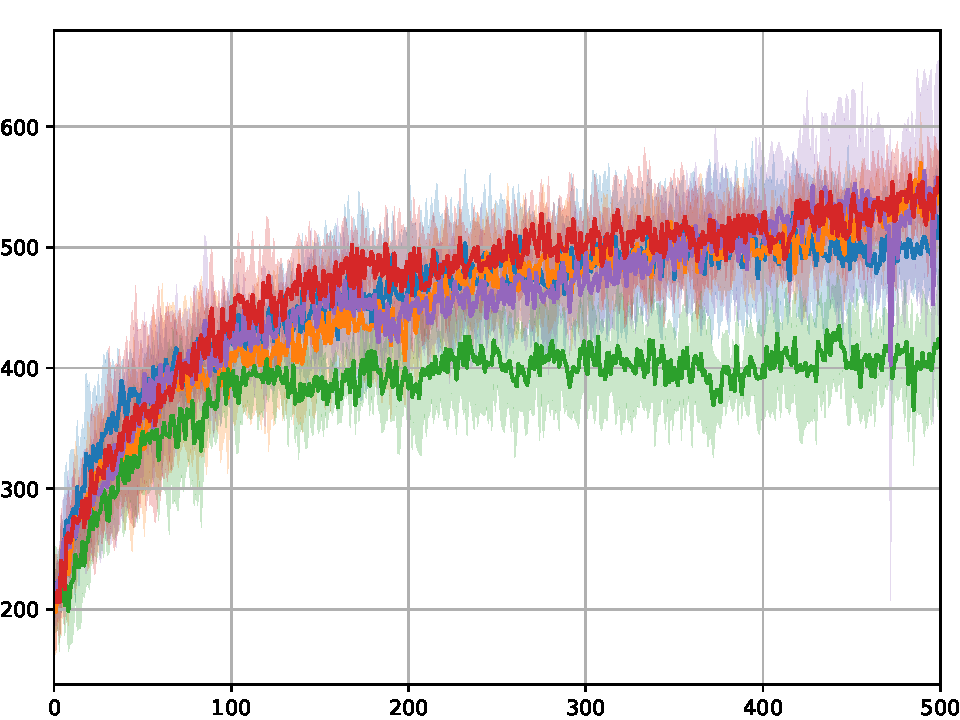
\includegraphics[width=\textwidth]{emi_figures/Gravitar_all.pdf}
        \caption{\textit{Gravitar}}
    \end{subfigure}
    \begin{subfigure}{0.32\textwidth}
        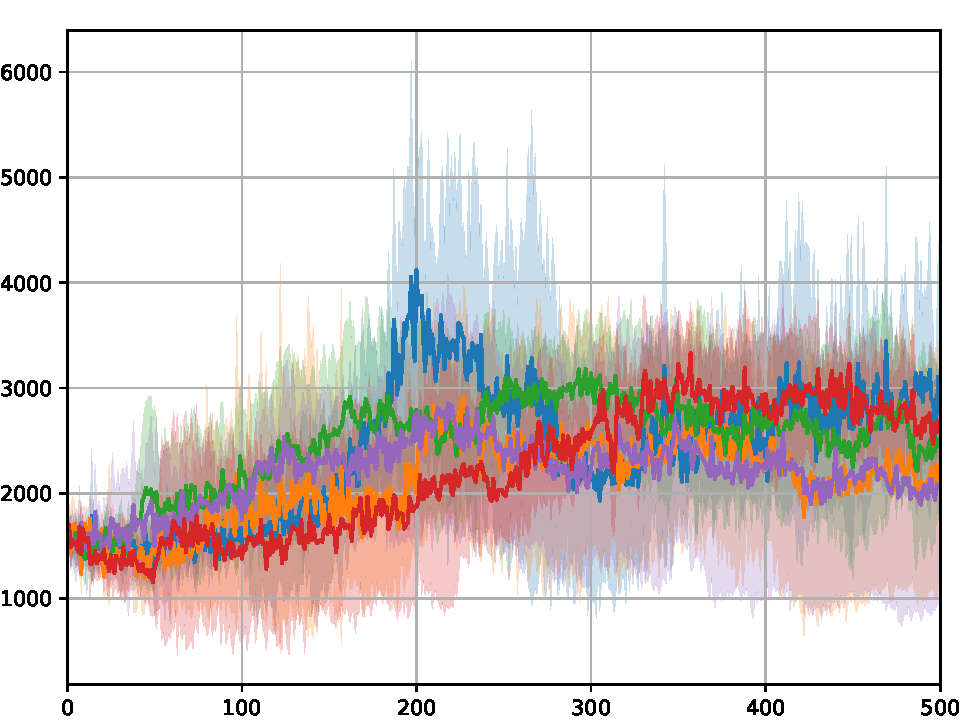
\includegraphics[width=\textwidth]{emi_figures/Solaris_all.pdf}
        \caption{\textit{Solaris}}
    \end{subfigure}
    \begin{subfigure}{0.32\textwidth}
        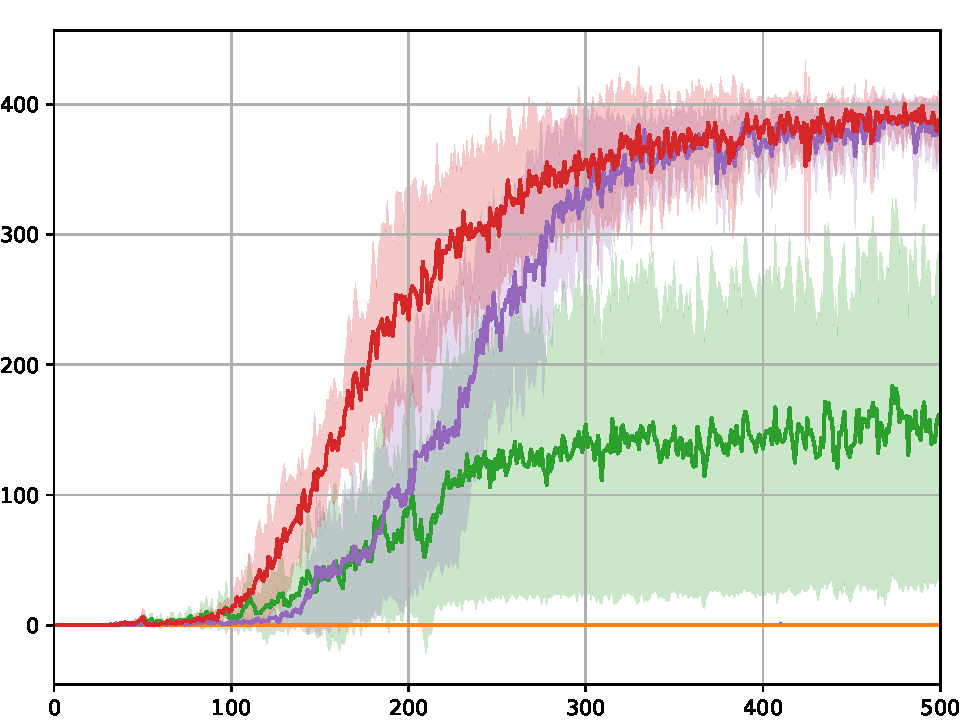
\includegraphics[width=\textwidth]{emi_figures/MontezumaRevenge_all.pdf}
        \caption{\textit{Montezuma's Revenge}}
    \end{subfigure}
  }
  \caption{Performance of EMI on sparse reward Atari environments compared to the baseline methods. The solid lines show the mean reward (y-axis) of 5 different seeds at each iteration (x-axis).}
\end{figure}
\end{frame}

%------------------------------------------------

\begin{frame}
\frametitle{Comparison of final performance}
\begin{table}[ht!]
\resizebox{\columnwidth}{!}{
\begin{tabular}{ |p{2.8cm}| >{\centering\arraybackslash}p{1.5cm} | >{\centering\arraybackslash}p{1.5cm}|  >{\centering\arraybackslash}p{1.5cm} | >{\centering\arraybackslash}p{1.5cm} | >{\centering\arraybackslash}p{2cm} | >{\centering\arraybackslash}p{1.5cm} | >{\centering\arraybackslash}p{1.5cm} |}
\hline
& EMI & EX2 & ICM  & RND & AE-SimHash & VIME & TRPO  \\
\hline
SwimmerGather& \textbf{0.438}& 0.200& 0 & 0 & 0.258& 0.196& 0\\
SparseHalfCheetah& \textbf{218}& 153.7& 1.4& 3.36 & 0.5& 98.0& 0\\
\hline
Freeway & \textbf{33.8}& 27.1& 33.6& 33.3 & 33.5& -& 26.7\\

Frostbite & \textbf{7002}& 3387& 4465& 2227 & 5214& -& 2034\\

Venture & 646 & 589& 418& \textbf{707} & 445& -& 263\\

Gravitar & \textbf{558}& 550& 424& 546 & 482& -& 508\\

Solaris & 2688& 2276& 2453& 2051 & \textbf{4467}& -& 3101\\

Montezuma & \textbf{387}& 0& 161& 377 & 75& -& 0\\
\hline

 \hline
\end{tabular}
}
\caption{Mean reward comparison with baseline methods. We compare EMI with EX2, ICM, RND, AE-SimHash, VIME, and vanilla TRPO. The EMI, EX2, ICM, RND, and TRPO columns show the mean reward of 5 different seeds. The AE-SimHash and VIME columns show the results from the original papers. The results of MuJoCo experiments are reported at 5M and 100M time steps respectively. The results of Atari experiments are reported at 50M time steps.}
\end{table}
\end{frame}



%------------------------------------------------

\begin{frame}
\frametitle{Learned EMI embeddings}
  \begin{figure}[h]
    \centering
    \includegraphics<1>[width=\textwidth]{emi_figures/figure_paths_emb_sparsehalfcheetah_1.pdf}
    \includegraphics<2>[width=\textwidth]{emi_figures/figure_paths_emb_sparsehalfcheetah_2.pdf}
    \includegraphics<3>[width=\textwidth]{emi_figures/figure_paths_emb_sparsehalfcheetah_3.pdf}
    \includegraphics<4>[width=\textwidth]{emi_figures/figure_paths_emb_sparsehalfcheetah_4.pdf}
    \includegraphics<5>[width=\textwidth]{emi_figures/figure_paths_emb_sparsehalfcheetah_5.pdf}
    \caption{Example paths in and our state embeddings for \textit{SparseHalfCheetah}. Note that we did not use any dimensionality reduction techniques.}
  \end{figure}
\end{frame}

%------------------------------------------------

\begin{frame}
\frametitle{Learned EMI embeddings}
  \begin{figure}[h]
    \centering
    \includegraphics<1>[width=\textwidth]{emi_figures/figure_paths_emb_montezuma_1.pdf}
    \includegraphics<2>[width=\textwidth]{emi_figures/figure_paths_emb_montezuma_2.pdf}
    \includegraphics<3>[width=\textwidth]{emi_figures/figure_paths_emb_montezuma_3.pdf}
    \includegraphics<4>[width=\textwidth]{emi_figures/figure_paths_emb_montezuma_4.pdf}
    \includegraphics<5>[width=\textwidth]{emi_figures/figure_paths_emb_montezuma_5.pdf}
    \includegraphics<6>[width=\textwidth]{emi_figures/figure_paths_emb_montezuma_6.pdf}
    \includegraphics<7>[width=\textwidth]{emi_figures/figure_paths_emb_montezuma_7.pdf}
    \includegraphics<8>[width=\textwidth]{emi_figures/figure_paths_emb_montezuma_8.pdf}
    \includegraphics<9>[width=\textwidth]{emi_figures/figure_paths_emb_montezuma_9.pdf}
    \includegraphics<10>[width=\textwidth]{emi_figures/figure_paths_emb_montezuma_10.pdf}
    \includegraphics<11>[width=\textwidth]{emi_figures/figure_paths_emb_montezuma_11.pdf}
    \caption{Example paths in and our state embeddings for \textit{Montezuma's Revenge}. Note that we did not use any dimensionality reduction techniques.}
  \end{figure}
\end{frame}

%------------------------------------------------

\begin{frame}
\frametitle{Learned EMI embeddings}
  \begin{figure}[h]
    \centering
    \includegraphics<1>[width=\textwidth]{emi_figures/figure_paths_emb_frostbite_1.pdf}
    \includegraphics<2>[width=\textwidth]{emi_figures/figure_paths_emb_frostbite_2.pdf}
    \includegraphics<3>[width=\textwidth]{emi_figures/figure_paths_emb_frostbite_3.pdf}
    \includegraphics<4>[width=\textwidth]{emi_figures/figure_paths_emb_frostbite_4.pdf}
    \includegraphics<5>[width=\textwidth]{emi_figures/figure_paths_emb_frostbite_5.pdf}
    \includegraphics<6>[width=\textwidth]{emi_figures/figure_paths_emb_frostbite_6.pdf}
    \includegraphics<7>[width=\textwidth]{emi_figures/figure_paths_emb_frostbite_7.pdf}
    \includegraphics<8>[width=\textwidth]{emi_figures/figure_paths_emb_frostbite_8.pdf}
    \includegraphics<9>[width=\textwidth]{emi_figures/figure_paths_emb_frostbite_9.pdf}
    \includegraphics<10>[width=\textwidth]{emi_figures/figure_paths_emb_frostbite_10.pdf}
    \includegraphics<11>[width=\textwidth]{emi_figures/figure_paths_emb_frostbite_11.pdf}
    \caption{Example paths in and our state embeddings for \textit{Frostbite}. Note that we did not use any dimensionality reduction techniques.}
  \end{figure}
\end{frame}

%------------------------------------------------
\begin{frame}
\frametitle{Sample videos}
  \begin{itemize} \itemsep=30pt
      \item A sample video of the EMI agent in \textit{SwimmerGather}: \url{https://youtu.be/HYJBcblCX50}.
      \item A sample video of the EMI agent in \textit{Montezuma's Revenge}: \url{https://youtu.be/pGun3EwaHug}.
  \end{itemize}
\end{frame}

%------------------------------------------------
%%\subsection{Conclusion} % Sections can be created in order to organize your presentation into discrete blocks, all sections and subsections are automatically printed in the table of contents as an overview of the talk
%------------------------------------------------

\begin{frame}
\frametitle{Conclusion}
  \begin{itemize} \itemsep=16pt
      \item We presented EMI, which is an exploration method that constructs embedding representation of states and actions that \textbf{does not rely on generative decoding of the full observation} that extracts predictive signals that can be used to guide exploration.\pause
      \item Our results on challenging tasks with sparse rewards show that EMI transfers to \textbf{a wide range of tasks}.
  \end{itemize}
\end{frame}


\section{Learning Discrete and Continuous Factors of Data via Alternating Disentanglement}

\begin{frame}
\frametitle{Disentanglement}
\begin{figure}
\centering
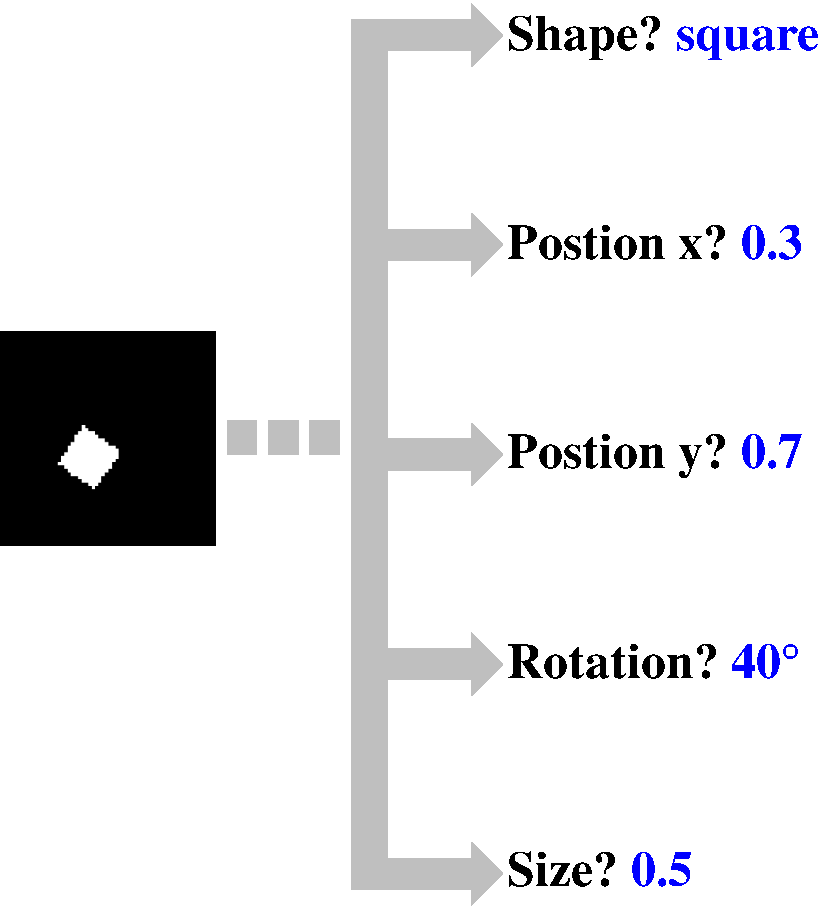
\includegraphics[width=0.6\linewidth]{dis_asset/disentanglement}
\end{figure}
\end{frame}

\begin{frame}
\frametitle{Motivation}
\begin{itemize}\itemsep=20pt
\item Our interest is to {\color{blue}{disentangle}} the underlying explanatory factors of data {\color{blue}{without any supervision.}}
\end{itemize}
\end{frame}

\begin{frame}
\frametitle{Motivation}
\begin{figure}
\centering
\only<1>{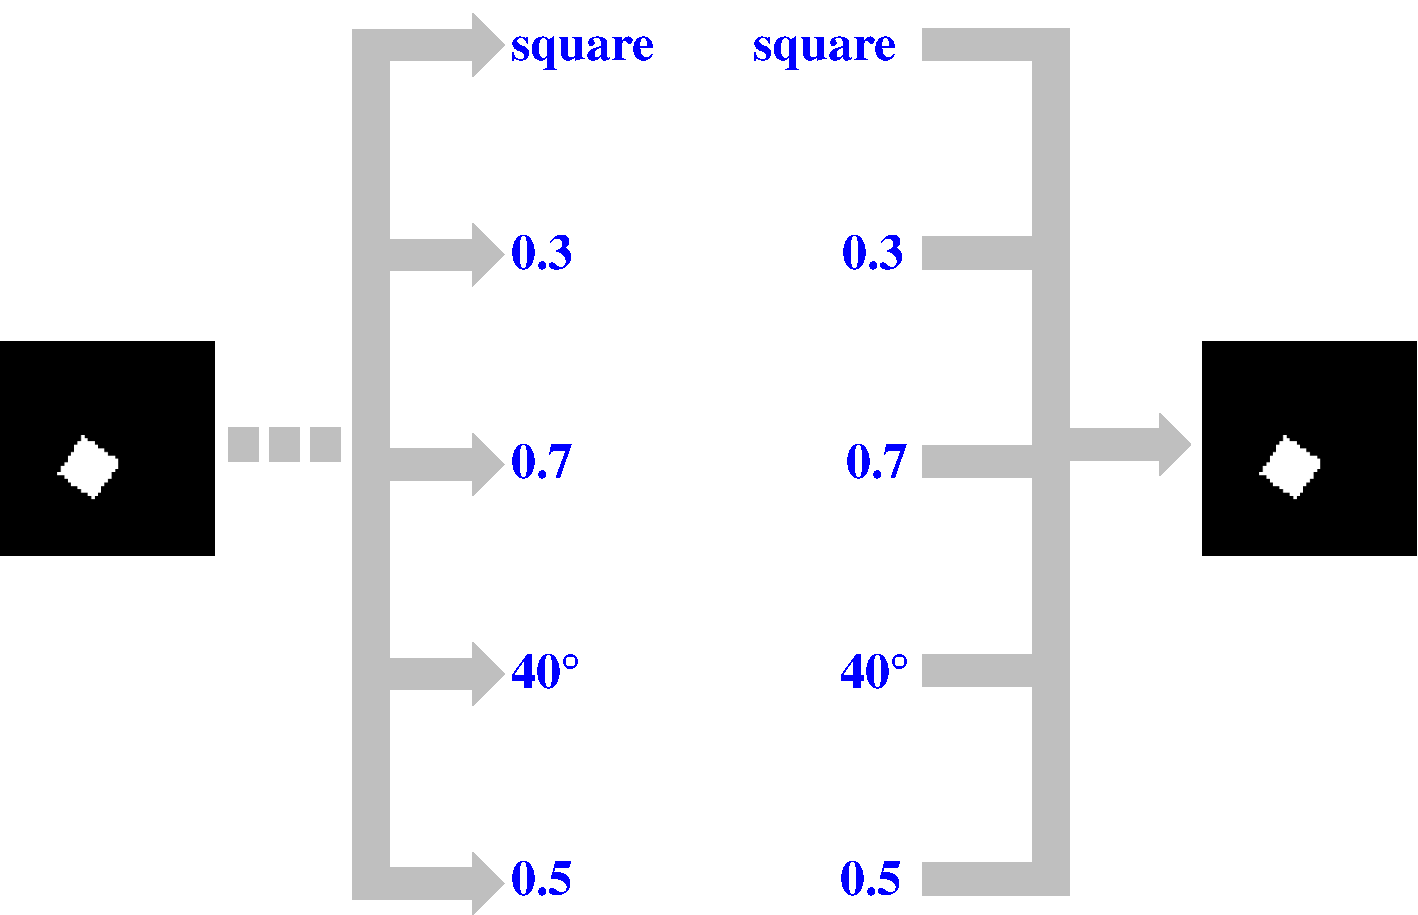
\includegraphics[page=1, width=\linewidth]{dis_asset/motivation}}%
\only<2>{\includegraphics[page=2, width=\linewidth]{dis_asset/motivation}}%
\only<3>{\includegraphics[page=3, width=\linewidth]{dis_asset/motivation}}%
\only<4>{\includegraphics[page=4, width=\linewidth]{dis_asset/motivation}}%
\only<5>{\includegraphics[page=5, width=\linewidth]{dis_asset/motivation}}%
\only<6>{\includegraphics[page=6, width=\linewidth]{dis_asset/motivation}}%
\only<7>{\includegraphics[page=7, width=\linewidth]{dis_asset/motivation}}%
\end{figure}
\end{frame}

\begin{frame}
\frametitle{Motivation}
\begin{itemize}\itemsep=20pt
\item Most recent methods focus on learning only the {\color{blue}{continuous}} factors of variation. \pause
\item When modeling complex and high-dimensional data such as raw images, it becomes difficult to disentangle the {\color{blue}{discrete}} factors of data (\ie~ number of light sources, categorical shape of present objects) from {\color{blue}{continuous}} factors (\ie~ translation, rotation, color).\pause
\item We require a stable disentanglement framework to capture {\color{blue}{continuous}} and {\color{blue}{discrete}} factors at the same time.
\end{itemize}
\end{frame}


\begin{frame}
\frametitle{Motivation}
\begin{figure}
\centering
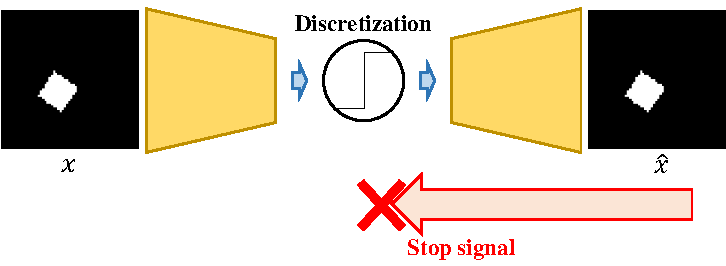
\includegraphics[page=1, width=\linewidth]{dis_asset/discrete}%
\end{figure}
\begin{itemize}
    \item If we use a step function at the end of encoder for discrete representation, {\color{red}{back-propagation cannot provide the training signal}}, because the derivative of a step function is 0 almost everywhere. This property becomes problematic when training discrete representations. 
\end{itemize}
\end{frame}

\begin{frame}
\frametitle{Motivation}
\begin{itemize}\itemsep=20pt
\item {\color{blue}{Learning discrete representations}} is known as a challenging problem. However, {\color{blue}{learning continuous and discrete representations}} is a more challening problem.
%%\pause\item {\color{blue}{VAE}} framework guarantees a stable framework compared to GAN framework.
\end{itemize}
\end{frame}



\begin{frame}
\frametitle{Contributions}
\begin{itemize}\itemsep=20pt
        \item We propose a simple procedure for penalizing the {\color{blue}{total correlation}} without any extra {\color{blue}{discriminator network(FactorVAE)}}\footnote{{\color{blue}{Kim, H. and Mnih, A.}} Disentangling by factorising. {\color{gray}{ICML2018}}} or {\color{blue}{importance sampling}} \footnote{{\color{blue}{Chen, T. Q., Li, X., Grosse, R. B., and Duvenaud, D. K.}} Isolating sources of disentanglement in variational autoencoders. {\color{gray}{NIPS2018}}} in the {\color{blue}{$\beta$-VAE}} \footnote{{\color{blue}{Higgins, I., Matthey, L., Pal, A., Burgess, C., Glorot, X., Botvinick, M., Mohamed, S., and Lerchner, A.}} beta-vae: Learning basic visual concepts with a constrained variational framework. {\color{gray}{ICLR2017}}} framework.\pause
\item We propose an {\color{blue}{alternating disentanglement method}} to disentangle discrete and continuous factors without lumping both the continuous and discrete factors into a single latent vector.
\end{itemize}
\end{frame}

%%\subsection{Method}
\begin{frame}
\frametitle{$\beta$-VAE framework}
\begin{itemize}\itemsep=20pt
\item VAE is a latent variable model that pairs a top-down decoding generator ($\theta$) and a bottom-up encoding inference network ($\phi$).\pause
%%\item A variational lower bound of the marginal log-likelihood, $\mathbb{E}_{x \sim p(x)} \log p(x)$, is maximized.\pause
\item VAE objective or the variational lower bound is,
\begin{align}
\mathcal{L}(\theta,\phi) = \mathbb{E}_{x \sim p(x)} \big[&\mathbb{E}_{z \sim q_\phi(z \mid x)} \log p_\theta(x \mid z)- \beta D_\text{KL}\left(q_\phi(z \mid x) \parallel p(z)\right)\big],\nonumber
\end{align}
where $p(z)$ is the fully factorized standard normal prior.
%%\item Maximizing the objective can be viewed as maximizing the lower bound on the mutual information between the data $x$ and the latent code $z$ with the KL term.
%%\begin{align}
%%    I(x;z) - \beta \mathbb{E}_{x\sim p(x)}D_\text{KL}(q_\phi(z\mid x) \parallel p(z)) \nonumber
%%\end{align}
\end{itemize}
\end{frame}

\begin{frame}
\frametitle{$\beta$-VAE framework}
\begin{itemize}\itemsep=12pt
\item We can decompose KL regularizer term. Concretely,
\begin{align}
&\mathbb{E}_{x \sim p(x)} D_\text{KL}(q(z| x) ~||~ p(z))\nonumber \\
&~~~=I(x;z) + \underbrace{D_\text{KL}(q(z) \parallel \prod_j q(z_j))}_{=~\text{Total correlation},~ TC(z)} + \sum_j D_\text{KL}(q(z_j) \parallel p(z_j)),\nonumber
\end{align}
        where $q(z)(=\mathbb{E}_{p(x)}[q(z\!\mid\!x)])$ denotes the marginal posterior. 
\end{itemize}
\end{frame}

\begin{frame}
\frametitle{Total Correlation $TC(z)$}
\begin{itemize}\itemsep=20pt
\item Total correlation or $TC(z)$ is a popular measure quantifying the redundancy among a set of $m$ random variables. \pause
\item Multivariate version of mutual information $I(\cdot, \cdot)$
\begin{align}
I(z_1,z_2)= D_\text{KL}(q(z_1,z_2) \parallel q(z_1)q(z_2))=TC(z_{1:2})\nonumber
\end{align}
        \vspace{-2em}
\pause \item {\color{blue}{Penalizing TC}} leads the model to learn {\color{blue}{statistically independent factors}} in the data which is a crucial component in disentangled representations. 
%%\begin{align}
%%TC(z) = D_\text{KL}(q(z) \parallel \prod_j q(z_j)),\nonumber
%%\end{align}
\end{itemize}
\end{frame}

\begin{frame}
\frametitle{Limitation of $\beta$-VAE}
\begin{itemize}\itemsep=20pt
\item $\beta$-VAE objective is
\begin{align}
\mathbb{E}_{x \sim p(x)} \big[\mathbb{E}_{z \sim q_\phi(z \mid x)} \log p_\theta(x \mid z)- \beta D_\text{KL}\left(q_\phi(z \mid x) \parallel p(z)\right)\big].\nonumber
\end{align}
\item $\beta$-VAE sets $\beta > 1$ to penalize $TC(z)$ which leads to statistically independent and disentangled representations. \pause
\item However, it penalizes the mutual information($=I(x,z)$) between the data and the latent variables. 
%%    \footnote{
%%\begin{align}
%%&\mathbb{E}_{x \sim p(x)} D_\text{KL}(q(z| x) ~||~ p(z))\nonumber \\
%%&~~~=I(x;z) + \underbrace{D_\text{KL}(q(z) \parallel \prod_j q(z_j))}_{=~\text{Total correlation},~ TC(z)} + \sum_j D_\text{KL}(q(z_j) \parallel p(z_j)),\nonumber
%%\end{align}}
\end{itemize}
\end{frame}

\begin{frame}
\frametitle{Overview of our method}
\begin{figure}
\includegraphics[page=2, width=\linewidth]{dis_asset/arch}
\end{figure}
\end{frame} 

\begin{frame}
\frametitle{Our method}
\begin{prop}
The mutual information between a single random variable and the rest can be factorized as
\[I(z_{1:i-1}; z_i) = TC(z_{1:i}) - TC(z_{1:i-1})\]
\end{prop}
\begin{prop}
The mutual information between $x$ and partitions of $z = [z_1, z_2]$ can be factorized as,
\[I(x; [z_1, z_2]) = I(x;z_1) + I(x; z_2) - I(z_1; z_2)\]
\end{prop}
\end{frame}

\begin{frame}
\frametitle{Our method}
\begin{itemize}\itemsep=12pt
\item By proposition1,
\begin{align}
TC(z)&=\underbrace{TC(z_{1:2})}_{= I(z_1; z_2)} + \sum_{i=3}^m \left( \underbrace{TC(z_{1:i}) - TC(z_{1:i-1})}_{= I(z_{1:i-1}; z_i)} \right)\nonumber\\
&= \sum_{i=2}^m I(z_{1:i-1}; z_i).\nonumber
\end{align}
\pause
\item We aim at penalizing $TC(z)$ by sequentially penalizing the individual summand $I(z_{1:i-1};z_i)$.
\end{itemize}
\end{frame}

\begin{frame}
\frametitle{Our method}
\begin{itemize}\itemsep=20pt
\item By proposition2,
\begin{align}
&I(x;z_{1:i}) = I(x;z_{1:i-1}) + I(x;z_{i}) - I(z_{1:i-1};z_{i}).\nonumber\\
&~~~~\only<2,3>{\uparrow} \only<1>{\qquad\qquad\quad\uparrow} \only<2,3>{\qquad\qquad\quad\bullet\quad\qquad\qquad\uparrow\qquad\qquad\quad\downarrow}\nonumber
\end{align}
\item This factorization motivates a maximization algorithm sequentially updating the left hand side $I(x; z_{1:i})$ for all $i=2,\ldots,m$ which in turn minimizes each summand, $\mathbf{I(z_{1:i-1};z_i)}$.
\onslide<3->{\item Sequentially, we maximize $I(x;z_{1:i})$ by penalizing $z_{i+1:m}$ with high $\beta$ ($:=\beta_h$) and the others with small $\beta$ ($:=\beta_l$).}
\end{itemize}
\end{frame}

\begin{frame}
\frametitle{Our method}
\begin{figure}
\only<1>{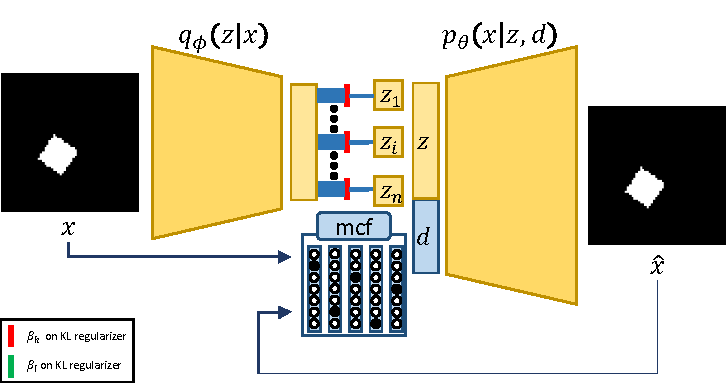
\includegraphics[page=1, width=\linewidth]{dis_asset/arch}}%
\only<2>{\includegraphics[page=2, width=\linewidth]{dis_asset/arch}}%
\only<3>{\includegraphics[page=3, width=\linewidth]{dis_asset/arch}}%
\only<4>{\includegraphics[page=4, width=\linewidth]{dis_asset/arch}}%
\end{figure}
\begin{itemize}
\item Every latent dimensions are heavily penalized with $\beta_h$. Each penalty on latent dimension is sequentially relieved one at a time with $\beta_l$ in a cascading fashion.
\end{itemize}
\end{frame} 

\begin{frame}
\frametitle{Graphical model}
\begin{figure}[bp]
\centering
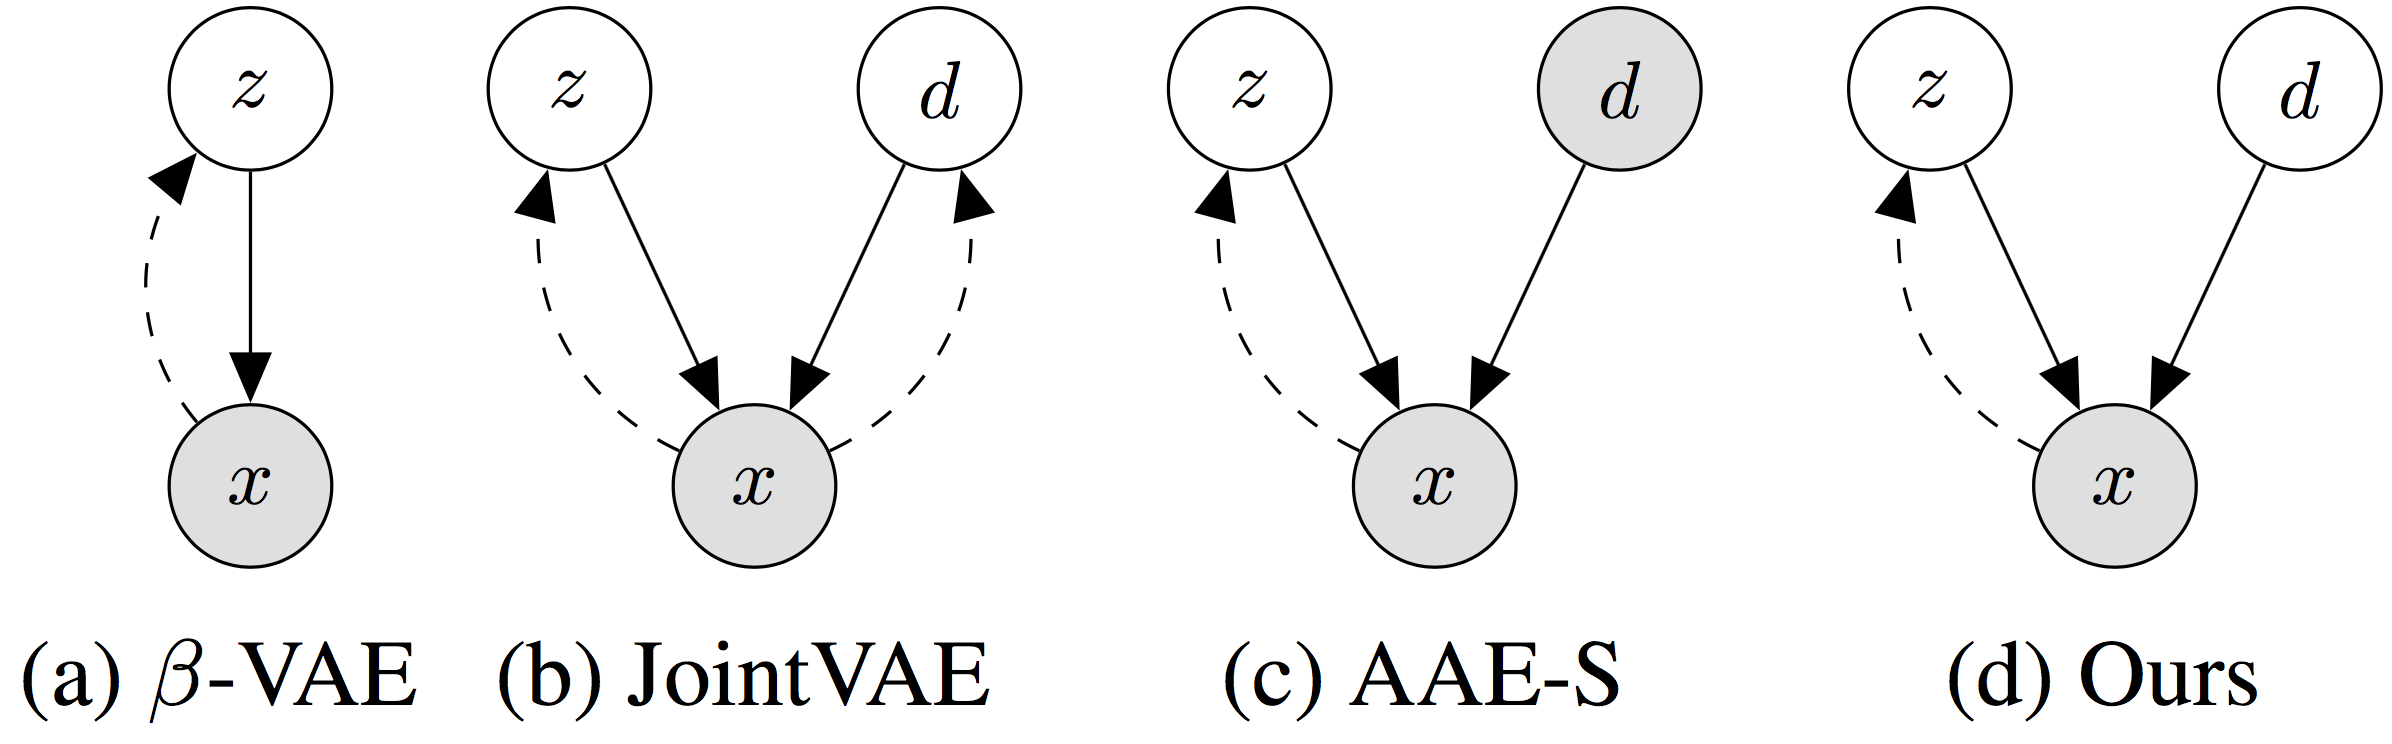
\includegraphics[width=1.0\linewidth]{dis_asset/graphical_model.png}
\caption{Graphical models view of $\beta$-VAE, JointVAE, AAE with supervised discrete variables(AAE-S), and our method. Solid lines denote the generative process and the dashed lines denote the inference process. $x,z,d$ denotes the data, continuous latent code, and the discrete latent code respectively.}
\end{figure}
\end{frame} 

\begin{frame}
\frametitle{Joint distribution}
\begin{itemize}
\item JointVAE
\begin{align}
    q(z,x,d) = p(x)q(z,d|x)\nonumber
\end{align}
\item AAE-S
\begin{align}
    q(z,x,d) = \begin{cases}p(x)q(z|x) & \text{if $d=y$} \\ 0 & \text{otherwise}\end{cases},\nonumber
\end{align}where $y$ is a provided ground truth discrete factors through supervision.
\item CascadeVAE
\begin{align}
    q(z,x,d) = \begin{cases}p(x)q(z|x) & \text{if $d = \argmax_{\hat{d}} p(x|z,\hat{d})$} \\0 &\text{otherwise}\end{cases}\nonumber
\end{align}
\end{itemize}
\end{frame}

\begin{frame}
\frametitle{Drawbacks of JointVAE}
\begin{itemize}\itemsep=12pt
\item 
\begin{align}
    q(z,x,d) = p(x)q(z,d|x)\nonumber
\end{align}
\item JointVAE can be viewed as  augmenting the continuous latent variables with discrete latent variables ($z=[z'; d]$) in the $\beta$-VAE framework.\pause
\item However, simply lumping the latent variables together offloads the entire burden of jointly modeling both the continuous and discrete factors to the variational posterior which can be very challenging.
\end{itemize}
\end{frame} 

\begin{frame}
\frametitle{AAE-S}
\begin{itemize}\itemsep=12pt
\item
\begin{align}
    q(z,x,d) = \begin{cases}p(x)q(z|x) & \text{if $d=y$} \\ 0 & \text{otherwise}\end{cases},\nonumber
\end{align}where $y$ is a provided ground truth discrete factors through supervision.
\item AAE have investigated learning continuous latent representations while providing the discrete factors through supervision(e.g. class labels in MNIST).\pause
\item Model can learn drastically better continuous representations when the burden of simultaneously modeling the continuous and discrete factors is relieved.
\end{itemize}
\end{frame} 

\begin{frame}
\frametitle{Our method}
\begin{itemize}\itemsep=12pt
\item
\begin{align}
    q(z,x,d) = \begin{cases}p(x)q(z|x) & \text{if $d = \argmax_{\hat{d}} p(x|z,\hat{d})$} \\0 &\text{otherwise}\end{cases}\nonumber
\end{align}
\item Inspired by these findings, our idea is to alternate between finding the most likely discrete configuration of the variables given the continuous factors, and updating the parameters ($\phi,\theta$) given the discrete configurations. 
\end{itemize}
\end{frame} 

\begin{frame}
\frametitle{Alternating minimization scheme}
    \begin{itemize}
\item Our goal is to maximize the variational lower bound of the following objective,
\small
\begin{align}
&\mathcal{L}(\theta,\phi)=I(x; [z,d]) - \beta \mathbb{E}_{x\sim p(x)} D_\text{KL}(q_\phi(z \mid x) \parallel p(z))-\lambda D_\text{KL} (q(d) \parallel p(d))\nonumber\\
& \geq H(x)+\int \sum_d q(x,z,d) \log q_{\theta, \phi}(x|z,d) dz dx\nonumber\\
&~~-\beta \mathbb{E}_{x\sim p(x)} D_\text{KL}(q_\phi(z \mid x) \parallel p(z)) - \lambda D_\text{KL} (q(d) \parallel p(d))\nonumber\\
&\geq H(x)+\mathbb{E}_{x\sim p(x)}[\mathbb{E}_{z,d\sim q_{\phi, \theta}(\cdot | x)}[\log p_{\theta}(x|z,d)]]\nonumber\\
&\quad-\beta \mathbb{E}_{x\sim p(x)} D_\text{KL}(q_\phi(z \mid x) \parallel p(z))- \lambda (S\mathbb{E}_{d, d' \sim q(d)}[\mathds{1}(d=d')]-1).\nonumber
\end{align}
    \end{itemize}
\end{frame}

\begin{frame}
\frametitle{Alternating minimization scheme}
\begin{itemize}\itemsep=12pt
\item Note the lower bound has an inner maximization step over the discrete factors embedded in the variational posterior.
\item Data is sampled $x^{(i)} \in \mathcal{X}, i=1, \ldots, n$.
\item The continuous latent variables($z^{(i)}$) are samples from the decoder $q_\phi(\cdot \mid x^{(i)})$. 
\item The discrete latent variables are represented using one-hot encodings of each variables $d^{(i)} \in \{e_1, \ldots, e_S\}$.
\end{itemize}
\end{frame}

\begin{frame}
\frametitle{Alternating minimization scheme}
\begin{itemize}
\item
    After rearranging the terms, we arrive at the following optimization problem.
\begin{align}
&\maximize_{\theta, \phi} \left(\underbrace{\maximize_{d^{(1)},\ldots d^{(n)}} \sum_{i=1}^n {u_\theta^{(i)}}^\intercal d^{(i)} - \lambda' \sum_{i\neq j} {d^{(i)}}^\intercal d^{(j)}}_{:= \mathcal{L}_{LB}(\theta, \phi)} \right)\nonumber\\
&\qquad\qquad\quad - \beta \sum_{i=1}^n D_{KL}(q_\phi(z|x^{(i)})||p(z))\nonumber\\
&\text{\ \  subject to }~~ \| d^{(i)} \|_1 = 1,~ d^{(i)} \in \{0,1\}^S,~ \forall i, \nonumber
\end{align}
where $u_\theta^{(i)}$ denotes the vector of the  likelihood $\log p_\theta(x^{(i)}|z^{(i)}, e_k)$ evaluated at each $k \in [S]$.
        
\end{itemize}
\end{frame}

\begin{frame}
\frametitle{Alternating minimization scheme}
\begin{itemize}
    \item The inner maximization problem $\mathcal{L}_{LB}(\theta, \phi)$  over the discrete variables $[d^{(1)},\ldots,d^{(n)}]$ subject to the sparsity equality constraints can be exactly solved in polynomial time via \emph{minimum cost flow}(mcf) without  continuous relaxation \footnote{ {\color{blue}{Jeong, Y. and Song, H. O.}} Efficient end-to-end learning for quantizable representations. {\color{gray}{ICML2018}} }. 
\end{itemize}
\end{frame}

\begin{frame}
\frametitle{Our method}
\begin{figure}
\includegraphics[page=2, width=\linewidth]{dis_asset/arch}
\caption{Architecture of CascadeVAE}
\end{figure}
\end{frame} 

%%\subsection{Experiments}
\begin{frame}
\frametitle{Pseudocode}
\begin{algorithm}[H]
\caption{CascadeVAE}
\footnotesize
\begin{algorithmic}[1]
\INPUT Data $\{x^{(i)}\}_{i=1}^N$, Encoder($q_\phi$), Decoder($p_\theta$), $\beta_l, \beta_h$, $r, t_d$, optimizer $g$
\STATE Initialize parameters $\phi, \theta$.
\STATE Set $\beta_j=\beta_h,~$ $\forall j$ and $d^{(i)}=0,$ $~~\forall i\in [N]$
\STATE Set $j=1$.
\FOR{$t=1,\ldots,$MAXITER}
\STATE \textbf{if} $t$ is a multiple of $r$
\STATE $~~~$Switch $\beta_j$ to $\beta_l$ and $j\leftarrow j+1$
\STATE Randomly select batch $\{x^{(i)}\}_{i \in \mathcal{B}}$
\STATE Sample $z^{(i)}_\phi \sim q_{\phi}(z|x^{(i)})$ $\forall i \in \mathcal{B}$ 
\STATE \textbf{if} $t>t_d$
\STATE $~~~$ Update $u_\theta^{(i)}$ by computing $\log p_\theta(x^{(i)}|z^{(i)}, e_k)$ $\forall k$
\STATE $~~~$ Compute $\mathcal{L}_{LB}(\theta, \phi)$ by solving for the optimal \\
\qquad assignment $\{d^{(i)}\}_{i\in \mathcal{B}}$ via minimum cost flow 
\STATE $\theta, \phi \leftarrow g\left(\nabla_{\theta,\phi} \mathcal{L}_{LB}(\theta,\phi)\right)$
\ENDFOR
\end{algorithmic}
\end{algorithm}
\end{frame}


\begin{frame}
\frametitle{Notation}
\begin{itemize}\itemsep=12pt
\item We denote our method without the discrete variables as \textbf{CascadeVAE-C}.
\item We denote our full method as \textbf{CascadeVAE}. 
\item We evaluate with disentanglement score introduced in \textbf{FactorVAE} and unsupervised classification accuracy.
\item Baselines are \textbf{$\beta$-VAE, JointVAE, FactorVAE}
\end{itemize}
\end{frame}

\begin{frame}
\frametitle{dSprites Dataset}
\begin{itemize}\itemsep=20pt
\item This dataset is used to assess the disentanglement properties of unsupervised learning methods.\pause
\item There are 6 ground truth independent latent factors\\
    (e.g. color, shape, scale, orientation, position x, position y).\pause
\item There are $737280$ $(=1\times3\times6\times40\times32\times32)$ images.
\end{itemize}
\end{frame}

\begin{frame}
\frametitle{dSprites Dataset Example}
\begin{columns}
\begin{column}{0.35\textwidth}
\begin{figure}
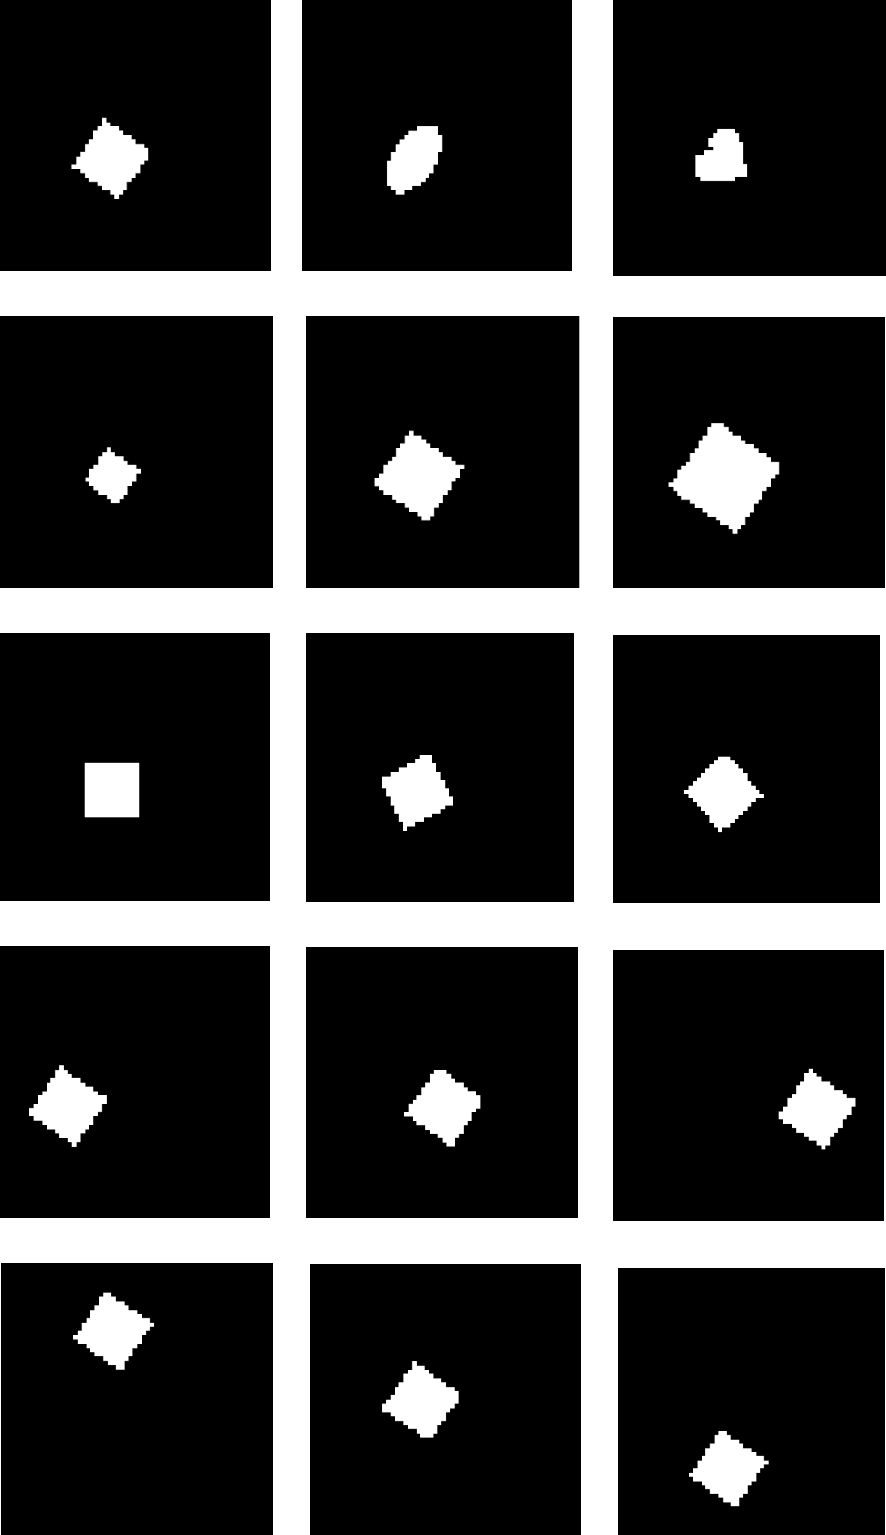
\includegraphics[width=\linewidth]{dis_asset/dsprites}
\end{figure}
\end{column}
\begin{column}{0.65\textwidth}
\begin{itemize}\itemsep=26pt
\item Shape {\color{red}{(discrete)}} : square, ellipse, heart
\item Scale: 6 values linearly spaced in $[0.5, 1]$
\item Orientation: 40 values in $[0, 2\pi]$
\item Position X: 32 values in $[0, 1]$
\item Position Y: 32 values in $[0, 1]$

\end{itemize}
\end{column}
\end{columns}

\end{frame}

\begin{frame}
\frametitle{Quantitative results on dSprites}
\begin{columns}
\begin{column}{0.5\textwidth}
\begin{table}[htbp]
\centering
\fontsize{9pt}{9.5pt}\selectfont
\begin{tabular}{rc rr}
\addlinespace[-\aboverulesep]
\toprule
\multicolumn{1}{c}{Method}&m&\multicolumn{1}{c}{Mean (std)}&\multicolumn{1}{c}{Best}\\
\toprule
$\beta$ VAE\\($\beta=10.0$)& 5 & 70.11 (7.54)&84.62\\
($\beta=4.0$)& 10 &74.41 (7.68)&88.38\\
\midrule
FactorVAE& 5  &81.09 (2.63)&85.12\\
        & 10 &82.15 (0.88)&88.25\\
\midrule
CascadeVAE-C\\($\beta_l=0.7$)& 5  &81.69 (3.14)&88.38\\
    ($\beta_l=1.0$)& 10 &81.74 (2.97)&87.38\\
\midrule
\midrule
JointVAE & 6 &  74.51 (5.17)&91.75\\
        & 4 &  73.06 (2.18)&75.38\\
\midrule
CascadeVAE\\($\beta_l=1.0$)& 6 &90.49 (5.28)&\textbf{99.50}\\
($\beta_l=2.0$)& 4 &\textbf{91.34 (7.36)}&98.62\\
\bottomrule
\end{tabular}
\end{table}
\end{column}
\begin{column}{0.35\textwidth}
\begin{itemize}\itemsep=12pt
\item {\color{blue}{Disentanglement score}} is obtained from 10 different random seed each with the best hyperparameters. 
\item $m$ is the number of continous latent dimensions.
\end{itemize}
\end{column}
\end{columns}
\end{frame}


\begin{frame}
\frametitle{Quantitative results on dSprites}
\begin{columns}
\begin{column}{0.5\textwidth}
\begin{table}[htbp]
\fontsize{9pt}{9.5pt}\selectfont
\centering
\begin{tabular}{rc ll}
\addlinespace[-\aboverulesep]
\toprule
\multicolumn{1}{c}{Method}&m&\multicolumn{1}{c}{Mean (std)}&\multicolumn{1}{c}{Best}\\
\toprule
JointVAE & 6&44.79 (3.88) &53.14\\
        &  4&43.99 (3.94) &54.11\\
\midrule
CascadeVAE &6&\textbf{78.84 (15.65)}& \textbf{99.66}\\
                &4&76.00 (22.16)& 98.72\\
\bottomrule
\end{tabular}
\end{table}
\end{column}
\begin{column}{0.4\textwidth}
\begin{itemize}\itemsep=12pt
\item {\color{blue}{Unsupervised classification accuracy}} when size of discrete variable is 3.
\item Random chance : $33.33$.
\end{itemize}

\end{column}
\end{columns}
\end{frame}


%%\begin{frame}
%%\frametitle{Quantitative results on dSprites}
%%\begin{figure}[]
%%\centering
%%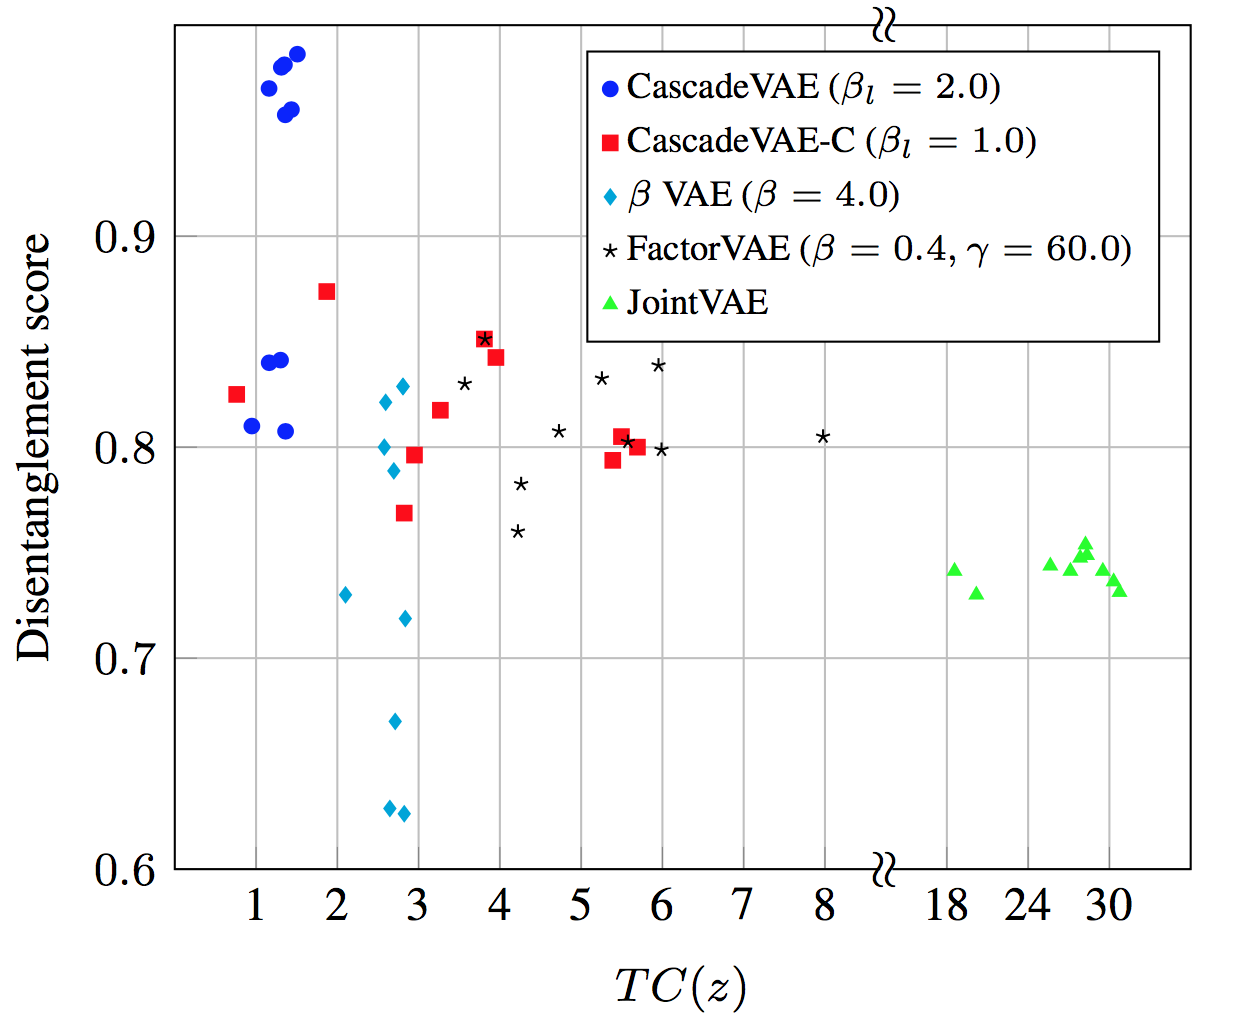
\includegraphics[width=0.65\linewidth]{tc_score.png}
%%\end{figure}
%%\end{frame}

%%\begin{frame}
%%\frametitle{Qualitative results on dSprites}
%%\begin{figure}
%%\centering
%%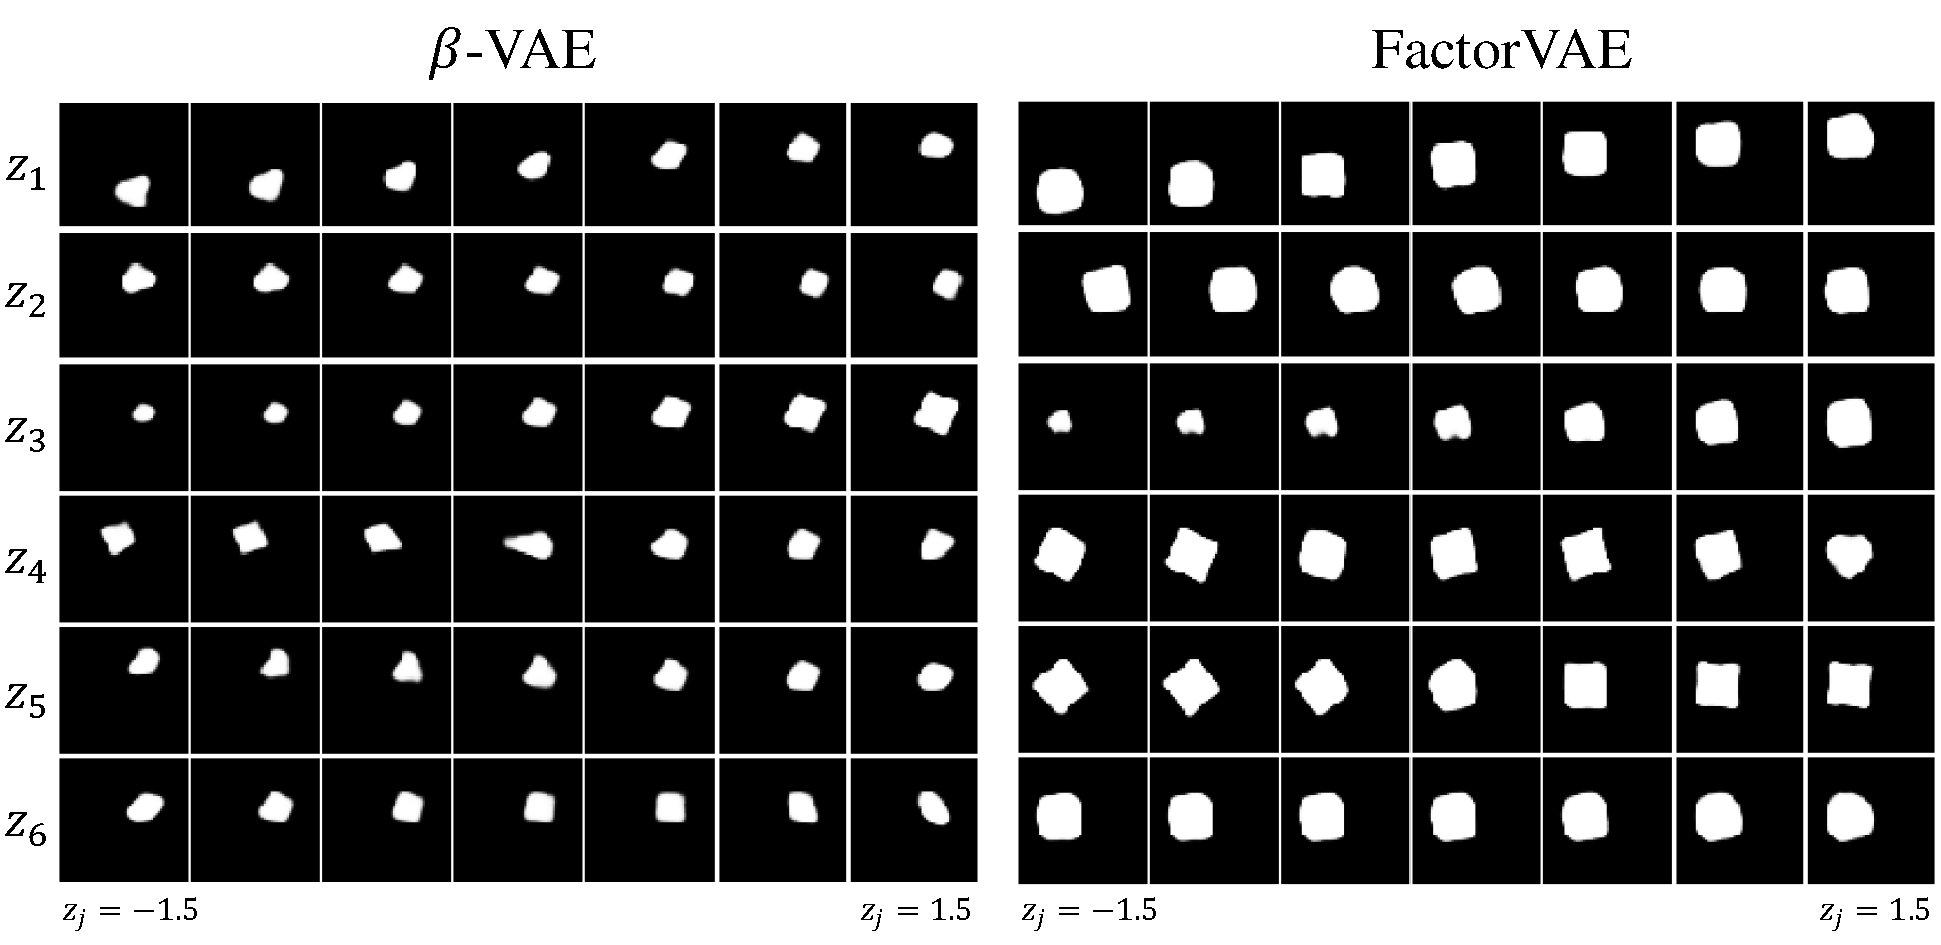
\includegraphics[width=0.9\textwidth,center]{dsprites_beta_factor}
%%\end{figure}
%%\end{frame}

\begin{frame}
\frametitle{Latent dimension traversal in dSprites}
\begin{itemize}\itemsep=8pt
\item $\beta$-VAE\\
$\mathbf{\qquad\quad z_1\qquad\qquad~z_2\qquad\qquad~z_3\qquad\qquad~z_4\qquad\qquad~~z_5}$
\vspace{-0.6em}
\begin{figure}
\centering
\only<1>{
\includegraphics[width=0.9\textwidth,center]{vae_gif/vae-0.png}}%
\only<2>{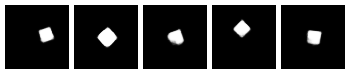
\includegraphics[width=0.9\textwidth,center]{vae_gif/vae-5.png}}%
\only<3>{
\includegraphics[width=0.9\textwidth,center]{vae_gif/vae-10.png}}%
\only<4>{
\includegraphics[width=0.9\textwidth,center]{vae_gif/vae-15.png}}%
\only<5>{
\includegraphics[width=0.9\textwidth,center]{vae_gif/vae-20.png}}%
\only<6>{
\includegraphics[width=0.9\textwidth,center]{vae_gif/vae-25.png}}%
\only<7>{
\includegraphics[width=0.9\textwidth,center]{vae_gif/vae-30.png}}%
\only<8>{
\includegraphics[width=0.9\textwidth,center]{vae_gif/vae-35.png}}%
\only<9>{
\includegraphics[width=0.9\textwidth,center]{vae_gif/vae-40.png}}%
\only<10>{
\includegraphics[width=0.9\textwidth,center]{vae_gif/vae-45.png}}
\end{figure}
\item FactorVAE\\
$\mathbf{\qquad\quad z_1\qquad\qquad~z_2\qquad\qquad~z_3\qquad\qquad~z_4\qquad\qquad~~z_5}$
\vspace{-0.6em}
\begin{figure}
\only<1>{
\includegraphics[width=0.9\textwidth,center]{factor_gif/factor-0.png}}%
\only<2>{
\includegraphics[width=0.9\textwidth,center]{factor_gif/factor-5.png}}%
\only<3>{
\includegraphics[width=0.9\textwidth,center]{factor_gif/factor-10.png}}%
\only<4>{\includegraphics[width=0.9\textwidth,center]{factor_gif/factor-15.png}}%
\only<5>{\includegraphics[width=0.9\textwidth,center]{factor_gif/factor-20.png}}%
\only<6>{\includegraphics[width=0.9\textwidth,center]{factor_gif/factor-25.png}}%
\only<7>{\includegraphics[width=0.9\textwidth,center]{factor_gif/factor-30.png}}%
\only<8>{\includegraphics[width=0.9\textwidth,center]{factor_gif/factor-35.png}}%
\only<9>{\includegraphics[width=0.9\textwidth,center]{factor_gif/factor-40.png}}%
\only<10>{\includegraphics[width=0.9\textwidth,center]{factor_gif/factor-45.png}}
\end{figure}
\end{itemize}
\end{frame}

\begin{frame}
\frametitle{Latent dimension traversal in dSprites}
\begin{itemize}\itemsep=8pt
\item JointVAE\\
\end{itemize}
\begin{columns}
\begin{column}{0.07\textwidth}
\vspace{0.5em}\\
$\mathbf{d=[1, 0,  0]}$\\\vspace{3em}
$\mathbf{d=[0, 1, 0]}$\\\vspace{3em}
$\mathbf{d=[0, 0, 1]}$
\end{column}
\begin{column}{0.93\textwidth}
$\mathbf{\qquad\quad~z_1\qquad~~~z_2\qquad\quad~ z_3\qquad\quad\,z_4\qquad\quad\, z_5\qquad\quad\, z_6}$
\vspace{-1em}
\begin{figure}
\centering
\only<1>{\includegraphics[width=0.9\textwidth,center]{joint_gif/jointvae-0.png}}%
\only<2>{\includegraphics[width=0.9\textwidth,center]{joint_gif/jointvae-5.png}}%
\only<3>{\includegraphics[width=0.9\textwidth,center]{joint_gif/jointvae-10.png}}%
\only<4>{\includegraphics[width=0.9\textwidth,center]{joint_gif/jointvae-15.png}}%
\only<5>{\includegraphics[width=0.9\textwidth,center]{joint_gif/jointvae-20.png}}%
\only<6>{\includegraphics[width=0.9\textwidth,center]{joint_gif/jointvae-25.png}}%
\only<7>{\includegraphics[width=0.9\textwidth,center]{joint_gif/jointvae-30.png}}%
\only<8>{\includegraphics[width=0.9\textwidth,center]{joint_gif/jointvae-35.png}}%
\only<9>{\includegraphics[width=0.9\textwidth,center]{joint_gif/jointvae-40.png}}%
\only<10>{\includegraphics[width=0.9\textwidth,center]{joint_gif/jointvae-45.png}}
\end{figure}

\end{column}
\end{columns}

\end{frame}

\begin{frame}
\frametitle{Latent dimension traversal in dSprites}
\begin{itemize}\itemsep=8pt
\item CascadeVAE\\
\end{itemize}
\begin{columns}
\begin{column}{0.07\textwidth}
\vspace{0.5em}\\
$\mathbf{d=[1, 0,  0]}$\\\vspace{3em}
$\mathbf{d=[0, 1, 0]}$\\\vspace{3em}
$\mathbf{d=[0, 0, 1]}$
\end{column}
\begin{column}{0.93\textwidth}
$\mathbf{\qquad\quad~z_1\qquad~~~z_2\qquad\quad~ z_3\qquad\quad\,z_4\qquad\quad\, z_5\qquad\quad\, z_6}$
\vspace{-1em}
\begin{figure}
\centering
\only<1>{\includegraphics[width=0.9\textwidth,center]{cascade_gif/cascade-0.png}}%
\only<2>{\includegraphics[width=0.9\textwidth,center]{cascade_gif/cascade-5.png}}%
\only<3>{\includegraphics[width=0.9\textwidth,center]{cascade_gif/cascade-10.png}}%
\only<4>{\includegraphics[width=0.9\textwidth,center]{cascade_gif/cascade-15.png}}%
\only<5>{\includegraphics[width=0.9\textwidth,center]{cascade_gif/cascade-20.png}}%
\only<6>{\includegraphics[width=0.9\textwidth,center]{cascade_gif/cascade-25.png}}%
\only<7>{\includegraphics[width=0.9\textwidth,center]{cascade_gif/cascade-30.png}}%
\only<8>{\includegraphics[width=0.9\textwidth,center]{cascade_gif/cascade-35.png}}%
\only<9>{\includegraphics[width=0.9\textwidth,center]{cascade_gif/cascade-40.png}}%
\only<10>{\includegraphics[width=0.9\textwidth,center]{cascade_gif/cascade-45.png}}
\end{figure}
\end{column}
\end{columns}
\end{frame}


\begin{frame}
\frametitle{Quantitative results on MNIST}
\begin{columns}
\begin{column}{0.5\textwidth}
\begin{table}[htbp]
\centering
\fontsize{9pt}{9.5pt}\selectfont
\begin{tabular}{rc rr}
\addlinespace[-\aboverulesep]
\toprule
\multicolumn{1}{c}{Method}&m& \multicolumn{1}{c}{Mean (std)}&\multicolumn{1}{c}{Best}\\
\toprule
JointVAE & 10&68.57 (9.19) &82.30\\
        &  4&78.33 (7.18) &92.81\\
\midrule
CascadeVAE &10&81.41 (9.54)& \textbf{97.31}\\
           & 4&\textbf{84.19 (5.02)}& 96.39\\
\bottomrule
\end{tabular}
\end{table}
\end{column}
\begin{column}{0.4\textwidth}
\begin{itemize}\itemsep=12pt
\item {\color{blue}{Unsupervised classification accuracy}} when size of discrete variable is 10.
\item Random chance : $10.00$.
\end{itemize}

\end{column}
\end{columns}
\end{frame}


\begin{frame}
\frametitle{Qualitative results on MNIST}
\begin{figure}[bp]
\centering
\begin{subfigure}[t]{0.48\linewidth}
\centering
\includegraphics[width=0.8\linewidth]{dis_asset/mnist_slant.png}
\caption{Angle}
\end{subfigure}\hspace{0.005\linewidth}
\begin{subfigure}[t]{0.48\linewidth}
\centering
\includegraphics[width=0.8\linewidth]{dis_asset/mnist_width.png}
\caption{Width}
\end{subfigure}\hspace{0.005\linewidth}
\begin{subfigure}[t]{0.48\linewidth}
\centering
\includegraphics[width=0.8\linewidth]{dis_asset/mnist_style.png}
\caption{Stroke}
\end{subfigure}\hspace{0.005\linewidth}
\begin{subfigure}[t]{0.48\linewidth}
\centering
\includegraphics[width=0.8\linewidth]{dis_asset/mnist_thickness.png}
\caption{Thickness}
\end{subfigure}
\caption{ Latent traversals on MNIST. Images in a row has the same latent variables except the traversed variable.}
\end{figure}
\end{frame}

\begin{frame}
\frametitle{Qualitative results on MNIST}
\begin{figure}[bp]
\centering
\includegraphics[width=0.8\linewidth]{dis_asset/mnist_digit.png}
\caption{MNIST discrete latent space traversal. Images in a row has the same latent variables except discrete variable.}
\end{figure}
\end{frame}

\begin{frame}
\frametitle{Qualitative results on Chairs}
\begin{figure}[htbp]
\centering
\includegraphics[width=\linewidth]{dis_asset/chairs}
\caption{Latent space traversal on chairs dataset. The last row shows the latent traversal of the discrete factor of dimension 3 with the period of 3.}
\label{fig:chairs_latent_traversal}
\end{figure}
\end{frame}

%%\subsection{Conclusion}

\begin{frame}
\frametitle{Conclusion}
\begin{itemize}\itemsep=12pt
        \item We first propose an {\color{blue}{efficient procedure for implicitly penalizing the total correlation}} by {\color{red}{controlling the information flow on each variables}} without using extra discriminator networks or sampling procedures.
\item We show a method for jointly learning discrete and continuous latent variables in an alternating maximization framework where we alternate between {\color{blue}{finding the most likely discrete configurations based on the continuous latent variables}}, and {\color{blue}{updating the inference parameters based on the discrete variables}}. 
\end{itemize}
\end{frame}

\begin{frame}
\frametitle{Conclusion}
\begin{itemize}
    \item Our ablation study shows that {\color{blue}{information cascading}} and {\color{blue}{alternating maximization of discrete and continuous variables}}, provide complementary benefits and leads to the state of the art performance in 1) \textbf{disentanglement score}, and 2) \textbf{classification accuracy score} from the discrete inference network, compared to a number of recently proposed methods.
\end{itemize}
\end{frame}

\section{Parsimonious black-box adversarial attacks via efficient combinatorial optimization}

%%\subsection{Background} % Sections can be created in order to organize your presentation into discrete blocks, all sections and subsections are automatically printed in the table of contents as an overview of the talk
%------------------------------------------------
\setbeamercolor{block title}{use=structure,fg=white,bg=structure.fg!75!black}
\setbeamercolor{block body}{parent=normal text,use=block title,bg=block title.bg!15!bg}

\begin{frame}
\frametitle{What is adversarial attack?}
\begin{itemize}\itemsep=12pt
    \item Neural networks are highly vulnerable to adversarial examples which are generated by adding imperceptibly small noise to original image.
\end{itemize}
\begin{figure}
    \centering
    \includegraphics[scale=0.30]{figures/adversarial_attack.png}
    \label{fig:adversarial_attack}
\end{figure}
\vspace{-3em}
\end{frame}

\begin{frame}
\frametitle{Why is it dangerous?}
\vspace{1em}
\begin{itemize}\itemsep=12pt
    \item Adversarial examples raise issues that are critical to the safety of AI in the real world.
\end{itemize}
\vspace{-1em}
\begin{figure}
    \centering
    \includegraphics[scale=0.20]{figures/adversarial_example_stop_sign.png}
    \label{fig:adversarial_example}
\end{figure}
\footnote{\scriptsize https://www.pluribus-one.it/research/sec-ml/wild-patterns/}
\end{frame}

\begin{frame}
\frametitle{Formal definition}
\begin{itemize}\itemsep=12pt
    \item Suppose that we have a classifier $C(x)$ with corresponding loss function $\ell(x, y)$, where $x$ is an original image and $y$ is its corresponding label.\pause
    \item $x_{adv}$ is called an adversarial example of $x$ if
    \begin{align*}
    C(x_{adv}) \neq y ~~ \text{and} ~~ \norm{x_{adv}-x}_p \le \epsilon
    \end{align*}\pause
    \vspace{-1.5em}
    \item It can be reformulated as the following constrained optimization problem.
    \begin{align*}
    \maximize_{x_{adv}}~\ell(x_{adv}, y) ~~ \text{subject to} ~~ \norm{x_{adv}-x}_p \le \epsilon
    \end{align*}
    \vspace{-1.5em}
\end{itemize}
\end{frame}

\begin{frame}
\frametitle{Threat model}
\begin{figure}
    \centering
    \includegraphics[scale=0.15]{figures/threat_model.png}
    \label{fig:adversarial_attack}
\end{figure}\pause
\begin{itemize}\itemsep=12pt
    \item White-box attack
    \begin{itemize}
        \item Adversary can access to the model parameters and the corresponding loss gradient with respect to an input.
    \end{itemize}\pause
    \item Black-box attack
    \begin{itemize}
        \item Adversary can query an input to the model and receive the class prediction scores, but does not have access to the model parameters.
    \end{itemize}
\end{itemize}
\end{frame}
 

\begin{frame}
\frametitle{White-box attacks}
\textbf{Fast Gradient Sign Method}
\vspace{0.5em}
\begin{itemize}
    \item Compute the gradient of the loss function according to the input pixels. Perturbation is the signs of these derivative mutiplied by a smaller number $\epsilon$.
    \[x_{adv} = x + \epsilon \sign (\nabla_x \ell(\theta, x, y))\]
\end{itemize}\pause

\vspace{1em}
    
\textbf{Iterative Projected Gradient Sign Method}
\vspace{0.5em}
\begin{itemize}
    \item A variant of the fast gradient sign method, where instead of taking a single step size $\epsilon$, smaller steps $\alpha$ are taken.
    \[x^{t+1} = \Pi_{x+\epsilon}(x^t+\alpha \sign (\nabla_x \ell(\theta, x^t, y))\]
\end{itemize}

\footnote{\scriptsize Ian Goodfellow et al., \textit{Explaining and Harnessing Adversarial Examples, 2015}}
\footnote{\scriptsize Madry et al., \textit{Towards deep learning models resistent to adversarial attack, 2017}}
\end{frame}

\begin{frame}
    \frametitle{Black-box attacks}
    \begin{itemize}\itemsep=12pt
        \item Black-box attack is \textbf{much more challenging} than white-box attack since we cannot access to the gradient information of the target network.\pause
        \item Still, black-box attack is a more \textbf{realistic setting} since commercial classifiers like Clarifai usually offer only prediction scores.
    \end{itemize}
    
\end{frame}

\begin{frame}
\frametitle{Black-box attacks with gradient estimation}
Recent methods mostly aim at \textbf{estimating the true gradient signal} based on the input queries.\pause
\vspace{1em}
\begin{itemize}\itemsep=12pt
    \item \textbf{ZOO}\footnote{\scriptsize Chen, et al., \textit{Zoo: Zeroth order optimization based black-box attacks to deep neural networks without training substitute models, 2017}} computes the coordinate-wise numerical gradients by querying for central difference values and apply coordinate descent method.
    \[\hat g_i \coloneqq \frac{\partial \ell(x)}{\partial x_i} \approx \frac{\ell (x+\sigma e_i) - \ell (x-\sigma e_i)}{2\sigma}\] \vspace{-1.5em} \pause
    \item \textbf{NES}\footnote{\scriptsize Ilyas, et al., \textit{Black-box adversarial attacks with limited queries and information, 2018}} and \textbf{Bandits}\footnote{\scriptsize Ilyas, et al., \textit{Prior convictions: Black-box adversarial attacks with bandits and priors, 2018}} compute the vector-wise gradient estimate with random sampled vectors $\{u_i\}$ by $\frac{1}{\sigma n} \sum_{i}^{n}(\ell(x+\sigma u_i)-\ell(x-\sigma u_i))u_i$ and apply projected gradient descent.
\end{itemize}
\end{frame}

\begin{frame}
\frametitle{Black-box attacks with gradient estimation}
\begin{itemize}\itemsep=12pt
        \item However, these black-box attacks are \textbf{very susceptible to the choice of hyperparameters} such as the learning rate, decay rates, and the update rule.\pause
        \item If we can devise an algorithm which does not require estimating the gradient, it would be \textbf{free of the update hyperparameters} and thus be more applicable.
\end{itemize}
\end{frame}

%%\subsection{Problem formulation}

\begin{frame}
    \frametitle{Objective}
    \begin{itemize}\itemsep=20pt
        \item We focus on \textbf{black-box} attacks under $\boldsymbol\ell_{\boldsymbol\infty}$ \textbf{constraint} with access to the network prediction scores only.\pause
        \item We aim to propose a new attack method under above setting with higher performance and query efficiency.
    \end{itemize}
    
\end{frame}


\begin{frame}
\frametitle{Motivation}
\begin{itemize}\itemsep=12pt
    \item White-box attacks find an adversarial example by deriving the following first order Taylor approximation of the loss function.
    \begin{align*}
        \ell(x_{adv}, y) \approx \ell(x, y) + (x_{adv}-x)^\intercal \nabla_{x}\ell(x, y)
    \end{align*}\pause
    \item Then, the optimization problem becomes
    \begin{align*}
        \maximize_{\norm{x_{adv}-x}_\infty \le \epsilon}~\ell(x_{adv}, y) ~\implies~ \maximize_{\norm{x_{adv}-x}_\infty \le \epsilon}~x_{adv}^\intercal \nabla_{x}\ell(x, y)
    \end{align*}\pause
    \item We can theoretically characterize that an optimal solution of the problem will be attained at a vertex of the $\ell_\infty$ constraint. 
\end{itemize}
\end{frame}

\begin{frame}{Motivation}
\begin{figure}[t]
% Figure 1a
\begin{tikzpicture}
\begin{axis}[
% Figure size
width = 5.8cm,
height = 5.36cm,
% Plot style
ybar,
bar width=0.13cm,
% Grid
grid=major,
% Tick
tick pos=left,
tick label style={font=\small},
xtick={-8, -6, -4, -2, 0, 2, 4, 6, 8},
xticklabels={-8, -6, -4, -2, 0, 2, 4, 6, 8},
ytick={0, 0.1, 0.2, 0.4, 0.5, 0.6},
yticklabels={0, 1e-2, 2e-2, 0.3, 0.4, 0.5},
% Label
xlabel={Change in pixel value \\},
ylabel={Ratio},
xlabel style={font=\small, at={(0.5, -0.08)}, align=center},
ylabel near ticks,
ylabel style={font=\small, at={(-0.2, 0.5)}},
% Range
ymin=0,
ymax=0.6
]
\addplot coordinates
{(-8, 0.5478980457715396) (-6, 0.14003602798375706) (-4, 0.1750571040783898)  (-2, 0.0639938095868644) (0, 0.1985194319385593) 
(2, 0.0743456479519774) (4, 0.18316064177259883) (6, 0.14652575476694912) (8, 0.5539381124205508)};
\end{axis}
\node[font=\scriptsize] at (0.35, -0.70) {(-$\epsilon$)};
\node[font=\scriptsize] at (3.87, -0.70) {($\epsilon$)};
%\node[font=\scriptsize] at (-0.09, -0.37) {(-$\epsilon$)};
%\node[font=\scriptsize] at (2.83, -0.37) {($\epsilon$)};
\draw (0, 1.9) -- node[fill=white,inner sep=-1.25pt,outer sep=0,anchor=center]{$\approx$} (0, 1.9);
\draw (4.22, 1.9) -- node[fill=white,inner sep=-1.25pt,outer sep=0,anchor=center]{$\approx$} (4.22, 1.9);
\end{tikzpicture}
\hspace{2.3em}
\vspace{-0.5em}
\caption{Distribution of adversarial noise with white box PGD attack on Cifar-10 dataset with wide Resnet w32-10 adversarially trained network at $\ell_\infty$ ball radius $\epsilon=8$ in [0, 255] scale.}
\label{fig:noise_distribution}
\end{figure}
\end{frame}

\begin{frame}
\frametitle{Motivation}
\begin{itemize}\itemsep=12pt
    \item This characterization motivates us to consider a \textbf{discrete surrogate} to the problem as follows.
    \begin{align*}
        \maximize_{\norm{x_{adv}-x}_\infty \le \epsilon}~\ell(x_{adv}, y) ~ \implies \maximize_{x_{adv}-x \in \{-\epsilon, \epsilon\}^d}~\ell(x_{adv}, y)
    \end{align*}
    where $d$ denotes the number of pixels in the image $x$.
\end{itemize}
\end{frame}

\begin{frame}
\frametitle{Problem formulation}
\begin{itemize}\itemsep=20pt
\item Equivalently, the discrete problem can be reformulated as the following set maximization problem.
\begin{align*}
\maximize_{\mathcal{S} \subseteq \mathcal{V}}~ \left\{ F(\mathcal{S}) \triangleq \ell \left(x + \epsilon \sum_{i \in \mathcal{S}}e_i - \epsilon \sum_{i \notin \mathcal{S}}e_i, y \right) \right\}
\end{align*}
where $\mathcal{V}$ denotes the set of all pixel locations, $\mathcal{S}$ denotes the set of selected pixels with $+\epsilon$ perturbations, and $\mathcal{V} \setminus \mathcal{S}$ indicates the set of remaining pixels with $-\epsilon$ perturbations. \pause
\item Now, our goal is to find $\mathcal{S}$ that maximizes the objective set function.
\end{itemize}
\end{frame}

%%\subsection{Method}

\begin{frame}
\frametitle{Submodular function}
\begin{itemize}\itemsep=25pt
\item In general, maximizing a set function is NP-hard.\pause
\item However, many set functions that arise in machine learning problem often exhibit \textbf{submodularity}.
\end{itemize}
\end{frame}

\begin{frame}
\frametitle{Submodular function}
\begin{defn}
For a set function $F:2^{\mathcal{V}} \rightarrow \reals$, $\mathcal{S} \subseteq \mathcal{V}$, and $e \in \mathcal{V}$, the marginal gain of $F$ at $\mathcal{S}$ with respect to $e$ is defined by
\begin{align*}
\Delta(e \mid \mathcal{S}) := F(\mathcal{S}\cup\{e\})-F(\mathcal{S})
\end{align*}
\end{defn}
\begin{defn}
A function $F:2^{\mathcal{V}} \rightarrow \reals$ is submodular if for every $\mathcal{A} \subseteq \mathcal{B} \subseteq \mathcal{V}$ and $e \in \mathcal{V} \setminus \mathcal{B}$, it holds that
\begin{align*}
\Delta(e \mid \mathcal{A}) \geq \Delta(e \mid \mathcal{B})
\end{align*}
\end{defn}
\end{frame}

\begin{frame}
\frametitle{Greedy algorithm for submodular maximization}
\begin{itemize}\itemsep=12pt
\item Submodular functions have a diminishing return property where the marginal gain diminishes as the set size increases.\pause
\item Using this property, we can efficiently compute an approximate optimal solution of submodular function with \textbf{greedy-style algorithms}.\pause
\item These greedy-style algorithms provide theoretical guarantees with approximation bounds.
\vspace{0.5em}
\begin{itemize}\itemsep=6pt
    \item $(1-\frac{1}{e})$-approximation for monotone submodular function
    \item $\frac{1}{3}$-approximation for non-monotone submodular function
\end{itemize} 
\end{itemize}
\end{frame}

\begin{frame}
\frametitle{Local search algorithm}
\begin{itemize}\itemsep=10pt
    \item For non-monotone set functions, \textbf{local search algorithm}\footnote{Feige, et al., \textit{Maximizing non-monotone submodular functions, 2011}} performs better than standard greedy insertion algorithms.\pause
    \item The algorithm alternates between greedily inserting an element and removing an element while the marginal gain is strictly positive.\pause
\end{itemize}
\setcounter{algorithm}{0}
\begin{algorithm}[H]
\footnotesize
\caption{Local Search algorithm}
\label{alg:local_search}
\begin{algorithmic}[1]
\INPUT Objective set function $F$, Working set $\mathcal{S}$, Ground set $\mathcal{V}$
\FOR{$t=1,\ldots, \text{MAXITER}$}
\STATE Greedily insert elements of $\mathcal{V}$ into $\mathcal{S}$ while the marginal gain is strictly positive
\STATE Greedily delete elements from $\mathcal{S}$ while the marginal gain is strictly positive
\ENDFOR
\OUTPUT $\argmax\limits_{\mathcal{A} \in \{\mathcal{S}, \mathcal{V} \setminus \mathcal{S} \}} F(\mathcal{A})$
\end{algorithmic}
\end{algorithm}
\end{frame}

\begin{frame}
\frametitle{Black-box adversarial attack via local search optimization}
\begin{itemize}\itemsep=12pt
\item Unfortunately, our objective function may not be exactly submodular.\pause
\item However, we empirically found that running the local search algorithm on our objective function works to a substantial extent, with its performance comparable to well-known \textbf{white-box} attacks in some settings.\pause
\item Also, we proved that the algorithm also maintains a certain degree of performance when the submodularity is not severely deteriorated.
\end{itemize}
\end{frame}

\begin{frame}
    \frametitle{Black-box adversarial attack via local search optimization}
    \begin{figure}
        \centering
        \begin{tikzpicture}
            \begin{axis}[
            % Figure size
            width = 5.8cm,
    		height = 5.36cm,
            % Plot style
            %ybar,
            %bar width=0.02cm,
            % Grid
            grid=major,
            % Tick
            tick pos=left,
            tick label style={font=\scriptsize},
            ytick={-0.6, -0.4, -0.2, 0, 0.2, 0.4, 0.6},
            yticklabels={-0.6, -0.4, -0.2, 0, 0.2, 0.4, 0.6},
            % Label
            xlabel={Image index \\ (sorted by $f(\cdot)-f(x_{pgd})$)},
            xlabel style={font=\scriptsize, align=center},
            ylabel={$f(\cdot)-f(x_{pgd})$},
            ylabel near ticks,
            ylabel style={font=\scriptsize, at={(-0.15,0.5)}},
            % Range
            xmin=0,
            xmax=100,
            % Legend
            legend style={nodes={scale=0.7, transform shape}},
            % Mark
            no marks,
            ]
            \addplot+[const plot] table [x=x, y=ls, col sep=comma] {data/fig2_diff.csv};
            \addlegendentry{$x_{ls}$}
            \addplot+[const plot] table [x=x, y=g, col sep=comma] {data/fig2_diff.csv};
            \addlegendentry{$x_{g}$}
            \end{axis}
        \end{tikzpicture}
        \hspace{2.1em}
        \caption{$f(\cdot)-f(x_{pgd})$ values on random 100 samples on Cifar-10, where $x_{ls}$, $x_{g}$ and $x_{pgd}$ each denotes image perturbed by local search, greedy insertion and PGD method.}
    \end{figure}
    
\end{frame}

\begin{frame}
\frametitle{Black-box adversarial attack via local search optimization}
\setcounter{thm}{0}
\begin{thm}
Let $\mathcal{C}$ be an optimal solution for a function $F$ and $\mathcal{S}$ be the solution obtained by the local search algorithm. Then,
\begin{align*}
    2F(\mathcal{S})+F(\mathcal{V} \setminus \mathcal{S}) \ge  F(\mathcal{C}) + \xi \lambda_F(\mathcal{V}, 2),
\end{align*}
where 
\small
\begin{align*}
    \xi = \binom{|\mathcal{S} \setminus \mathcal{C}|}{2} + \binom{|\mathcal{C} \setminus \mathcal{S}|}{2} + |\overline{\mathcal{S} \cup \mathcal{C}}| \cdot |\mathcal{S}| + |\mathcal{C} \setminus \mathcal{S}| \cdot |\mathcal{S} \cap \mathcal{C}|
\end{align*}
\normalsize
and $\lambda_{F}(\cdot,\cdot)$ is the submodularity index\footnote{\scriptsize Zhou and Spanos, \textit{Casual meets submodular: Subset selection with directed information, 2016}} of $F$, which is a measure of the degree of submodularity.
\end{thm}
\end{frame}

\begin{frame}
\frametitle{Black-box adversarial attack via local search optimization}
\begin{itemize}\itemsep=12pt
\item Applying the local search algorithm on our objective set function, we obtain a set $\mathcal{S}$ of pixels to perturb the input $x$ with $+\epsilon$ and its complement $\mathcal{V} \setminus \mathcal{S}$ to perturb with $-\epsilon$.\pause
\item Finally, the perturbed image is computed as
\begin{align*}
x_{adv} \triangleq x + \epsilon \sum_{i \in \mathcal{S}}e_i - \epsilon \sum_{i \notin \mathcal{S}}e_i
\end{align*}
\end{itemize}
\end{frame}

\begin{frame}
\frametitle{Adversarial examples of our algorithm}
\begin{figure}
\centering
\includegraphics[scale=0.30]{figures/adv_image_examples.pdf}
\caption{The top row shows the original images and the bottom row shows the corresponding perturbed images from our method.}
\label{fig:adv_image_examples}
\end{figure}
\end{frame}

\begin{frame}
    \frametitle{Hierarchical approach for query efficiency}
    \begin{itemize}\itemsep=12pt
        \item Running the local search algorithm on the set of all pixels could be query inefficient.\pause
        \item To address this problem, we take a \textbf{hierarchical approach}, performing the local search on a coarse grid and use the results in the subsequent round on finer grid.
    \end{itemize}\pause
    \begin{figure}
        \centering
        \hspace*{-2.5em}
        \includegraphics[scale=0.35]{figures/hierarchical_1.png}
    \end{figure}
\end{frame}

\begin{frame}
    \frametitle{Hierarchical approach for query efficiency}
    \begin{itemize}\itemsep=12pt
        \item Running the local search algorithm on the set of all pixels could be query inefficient.
        \item To address this problem, we take a \textbf{hierarchical approach}, performing the local search on a coarse grid and use the results in the subsequent round on finer grid.
    \end{itemize}
    \begin{figure}
        \centering
        \hspace*{-2.5em}
        \includegraphics[scale=0.35]{figures/hierarchical_2.png}
    \end{figure}
\end{frame}

\begin{frame}
    \frametitle{Hierarchical approach for query efficiency}
    \begin{itemize}\itemsep=12pt
        \item Running the local search algorithm on the set of all pixels could be query inefficient.
        \item To address this problem, we take a \textbf{hierarchical approach}, performing the local search on a coarse grid and use the results in the subsequent round on finer grid.
    \end{itemize}
    \begin{figure}
        \centering
        \hspace*{-2.5em}
        \includegraphics[scale=0.35]{figures/hierarchical_3.png}
    \end{figure}
\end{frame}

\begin{frame}
    \frametitle{Hierarchical approach for query efficiency}
    \begin{itemize}\itemsep=12pt
        \item Running the local search algorithm on the set of all pixels could be query inefficient.
        \item To address this problem, we take a \textbf{hierarchical approach}, performing the local search on a coarse grid and use the results in the subsequent round on finer grid.
    \end{itemize}
    \begin{figure}
        \centering
        \hspace*{-2.5em}
        \includegraphics[scale=0.35]{figures/hierarchical_4.png}
    \end{figure}
\end{frame}

\begin{frame}
    \frametitle{Hierarchical approach for query efficiency}
    \begin{itemize}\itemsep=12pt
        \item Running the local search algorithm on the set of all pixels could be query inefficient.
        \item To address this problem, we take a \textbf{hierarchical approach}, performing the local search on a coarse grid and use the results in the subsequent round on finer grid.
    \end{itemize}
    \begin{figure}
        \centering
        \hspace*{-2.5em}
        \includegraphics[scale=0.35]{figures/hierarchical_5.png}
    \end{figure}
\end{frame}

%%\subsection{Experiments}

\begin{frame}
    \frametitle{Cifar-10}
    \begin{columns}
    \begin{column}{0.75\columnwidth}
    \begin{table}[htbp]
	\centering
	\small
	\begin{adjustbox}{max width=\columnwidth}
		\begin{tabular}{cccc|c}
			\toprule[1pt]
			\textbf{Method} &
			\vtop{\hbox{\strut \textbf{Success}}\hbox{\strut \textbf{rate}}} &
			\vtop{\hbox{\strut \textbf{Avg.}}\hbox{\strut \textbf{queries}}} &
			\vtop{\hbox{\strut \textbf{Med.}}\hbox{\strut \textbf{queries}}} &
			\vtop{\hbox{\strut \textbf{Avg. queries}}\hbox{\strut \textbf{(NES success)}}} \\
			\midrule
			PGD \scriptsize(white-box) & 47.2\% & 20 & - & - \\
			\midrule
			NES & 29.5\% & 2872 & 900 & 2872 \\
			Bandits & 38.6\% & 1877 & 459 & 520 \\
			\textbf{Ours} & \textbf{48.0}\% & \textbf{1261} & \textbf{356} & \textbf{247} \\
			\bottomrule[1pt]
		\end{tabular}
	\end{adjustbox}
    \caption{Results for $\ell_\infty$ untargeted attacks on Cifar-10. Maximum number of queries set to 20,000.}
    \end{table}
    \end{column}
    \end{columns}
\end{frame}

\begin{frame}
    \frametitle{ImageNet}
    \begin{columns}
    \begin{column}{0.50\columnwidth}
    \begin{table}[htbp]
	\centering
	\small
	\begin{adjustbox}{max width=\columnwidth}
		\begin{tabular}{cccc|c}
			\toprule[1pt]
			\textbf{Method} &
			\vtop{\hbox{\strut \textbf{Success}}\hbox{\strut \textbf{rate}}} &
			\vtop{\hbox{\strut \textbf{Avg.}}\hbox{\strut \textbf{queries}}} &
			\vtop{\hbox{\strut \textbf{Med.}}\hbox{\strut \textbf{queries}}} &
			\vtop{\hbox{\strut \textbf{Avg. queries}}\hbox{\strut \textbf{(NES success)}}} \\
			\midrule
			PGD \scriptsize{(white-box)} & 99.9 \% & 20 & - & - \\
			\midrule
			NES\textsuperscript{\textdagger} & 77.8\% & 1735 & - &1735 \\
			NES & 80.3\% & 1660 & 900 &1660 \\
			Bandits\textsuperscript{\textdagger} & 95.4\% & 1117 & - &703 \\
			Bandits & 94.9\% & 1030 & 286 & 603 \\
			\textbf{Ours} & \textbf{98.5\%} & \textbf{722} & \textbf{237} & \textbf{376} \\
			\bottomrule[1pt]
		\end{tabular}
	\end{adjustbox}
    \caption{Results for $\ell_\infty$ untargeted attacks on ImageNet. Maximum number of queries set to 10,000.}
    \end{table}
    \end{column}\pause
    \begin{column}{0.50\columnwidth}
    \begin{table}[htbp]
	\centering
	\small
	\begin{adjustbox}{max width=\columnwidth}
		\begin{tabular}{cccc|c}
			\toprule[1pt]
			\textbf{Method} &
			\vtop{\hbox{\strut \textbf{Success}}\hbox{\strut \textbf{rate}}} &
			\vtop{\hbox{\strut \textbf{Avg.}}\hbox{\strut \textbf{queries}}} &
			\vtop{\hbox{\strut \textbf{Med.}}\hbox{\strut \textbf{queries}}} &
			\vtop{\hbox{\strut \textbf{Avg. queries}}\hbox{\strut \textbf{(NES success)}}} \\
			\midrule
			PGD \scriptsize(white-box) & 100\% & 200 & - & - \\
			\midrule
			NES\textsuperscript{\textdagger}& 99.2\% & - & 11550 & - \\
			NES & 99.7\% & 16284 & 12650 & 16284 \\
			Bandits & 92.3\%  & 26421 & 18642 & 26421 \\
			\textbf{Ours} & \textbf{99.9\%} & \textbf{7485} & \textbf{5373}& \textbf{7371} \\
			\bottomrule[1pt]
		\end{tabular}
	\end{adjustbox}
    \caption{Results for $\ell_\infty$ targeted attacks on ImageNet. Maximum number of queries set to 100,000.}
    \end{table}
    \end{column}
    \end{columns}
\end{frame}

\begin{frame}
    \frametitle{Queries vs. Attack Success Rate plot}
    \begin{figure}[ht]
	\centering
	% Figure 5a
	\begin{subfigure}[t]{0.3\textwidth}
		\begin{tikzpicture}[scale=0.7]
		\begin{axis}[
		% Figure size
		width=5cm,
		height=4.8cm,
		% Plot style
		no marks,
		every axis plot/.append style={thick},
		% Grid
		grid=major,
		% Tick
		scaled ticks = false,
		ylabel near ticks,
		tick pos=left,
		tick label style={font=\small},
		xtick={0, 4000, 8000, 12000, 16000, 20000},
		xticklabels={0, 4k, 8k, 12k, 16k, 20k},
		ytick={0, 10, 20, 30, 40, 50},
		yticklabels={0, 10, 20, 30, 40, 50},
		% Label
		label style={font=\small},
		xlabel={The number of queries},
		ylabel={Success rate},
		% Range
		xmin=0,
		xmax=20000,
		ymin=0,
		ymax=55,
		]
		% Ours
		\addplot[red] table [x=base, y=Ours, col sep=comma]{data/cifar10_untargeted.csv};
		% NES
		\addplot[brown] table [x=base, y=NES, col sep=comma]{data/cifar10_untargeted.csv};
		% Bandits
		\addplot[blue] table [x=base, y=Bandits, col sep=comma]{data/cifar10_untargeted.csv};
		% PGD
		\draw[dashed] (0, 472) -- (20000, 472);
		\end{axis}
		\end{tikzpicture}
		\caption{Cifar-10, untargeted}\label{fig:cdf_cifar10}
	\end{subfigure}
	% Figure 5b
	\begin{subfigure}[t]{0.34\textwidth}
		\begin{tikzpicture}[scale=0.7]
		\begin{axis}[
		% Figure size
		width=5cm,
		height=4.8cm,
		% Plot style
		no marks,
		every axis plot/.append style={thick},
		% Grid
		grid=major,
		% Tick
		scaled ticks = false,
		ylabel near ticks,
		tick pos=left,
		tick label style={font=\small},
		xtick={0, 2000, 4000, 6000, 8000, 10000},
		xticklabels={0, 2k, 4k, 6k, 8k, 10k},
		ytick={0, 20, 40, 60, 80, 100},
		yticklabels={0, 20, 40, 60, 80, 100},
		% Label
		label style={font=\small},
		xlabel={The number of queries},
		ylabel={Success rate},
		ylabel style={at={(-0.2,0.5)}},
		% Range
		xmin=0,
		xmax=10000,
		ymin=0,
		ymax=110,
		% Legend
		legend style={legend columns=3, at={(1.22, 1.3)}},
		]
		% Ours
		\addplot[red] table [x=base, y=Ours, col sep=comma]{data/imagenet_untargeted.csv};
		\addlegendentry{Ours}
		% NES
		\addplot[brown] table [x=base, y=NES, col sep=comma]{data/imagenet_untargeted.csv};
		\addlegendentry{NES}
		% Bandtis
		\addplot[blue] table [x=base, y=Bandits, col sep=comma]{data/imagenet_untargeted.csv};
		\addlegendentry{Bandits}
		% PGD
		\draw[dashed] (0, 99.9) -- (10000, 99.9);
		\end{axis}
		\end{tikzpicture}
		\caption{ImageNet, untargeted}\label{fig:cdf_imagenet_untargeted}
	\end{subfigure}
	% Figure 5c
	\begin{subfigure}[t]{0.33\textwidth}
		\begin{tikzpicture}[scale=0.7]
		\begin{axis}[
		% Figure size
		width=5cm,
		height=4.8cm,
		% Plot style
		no marks,
		every axis plot/.append style={thick},
		% Grid
		grid=major,
		% Tick
		scaled ticks = false,
		ylabel near ticks,
		tick pos=left,
		tick label style={font=\small},
		xtick={0, 20000, 40000, 60000, 80000, 100000},
		xticklabels={0, 20k, 40k, 60k, 80k, 100k},
		ytick={0, 20, 40, 60, 80, 100},
		yticklabels={0, 20, 40, 60, 80, 100},
		% Label
		label style={font=\small},
		xlabel={The number of queries},
		ylabel={Success rate},
		ylabel style={at={(-0.2,0.5)}},
		% Range
		xmin=0,
		xmax=100000,
		ymin=0,
		ymax=110,
		]
		% Ours
		\addplot[red] table [x=base, y=Ours, col sep=comma]{data/imagenet_targeted.csv};
		% NES
		\addplot[brown] table [x=base, y=NES, col sep=comma]{data/imagenet_targeted.csv};
		% Bandtis
		\addplot[blue] table [x=base, y=Bandits, col sep=comma]{data/imagenet_targeted.csv};
		% PGD
		\draw[dashed] (0, 99.9) -- (10000, 99.9);
		\end{axis}
		\end{tikzpicture}
		\caption{ImageNet, targeted}\label{fig:cdf_imagenet_targeted}
	\end{subfigure}
	\vspace{-0.2em}
	\caption{(a) The cumulative distribution of the number of queries required for untargeted attack on Cifar-10, (b) untargeted attack on ImageNet (center), and (c) targeted attack on ImageNet. The dashed line indicates the success rate of white-box PGD. The results show that our method consistently finds successful adversarial images faster than the baseline methods.}
	\label{fig:cdf}
    \end{figure}
\end{frame}

\begin{frame}
    \frametitle{ImageNet with smaller $\epsilon$}
    \begin{figure}
        \centering
    	\begin{subfigure}[t]{0.48\textwidth}
    		\begin{tikzpicture}[scale=1.0]
    		\begin{axis}[
    		% Figure size
    		width=5cm,
    		height=4.8cm,
    		% Plot style
    		no marks,
    		every axis plot/.append style={thick},
    		% Grid
    		grid=major,
    		% Tick
    		scaled ticks = false,
    		ylabel near ticks,
    		tick pos = left,
        	tick label style={font=\small},
        	xtick={0, 2000, 4000, 6000, 8000, 10000},
        	xticklabels={0, 2k, 4k, 6k, 8k, 10k},
        	ytick={0, 20, 40, 60, 80, 100},
        	yticklabels={0, 20, 40, 60, 80, 100},
        	% Range
        	xmin=0,
        	xmax=10000,
        	ymin=0,
        	ymax=110,
        	% Label
        	xlabel={The number of queries},
        	ylabel={Success rate},
        	label style={font=\small},
        	ylabel near ticks,
        	ylabel style={at={(-0.15,0.5)}},
        	% Legend
        	legend style={legend columns=3, at={(2.0, 1.3)}},
    		]
    		% Ours
    		\addplot[red] table [x=base, y=Ours, col sep=comma]{data/imagenet_untargeted_0.01.csv};
    		\addlegendentry{Ours}
    		% NES
    		\addplot[brown] table [x=base, y=NES, col sep=comma]{data/imagenet_untargeted_0.01.csv};
    		\addlegendentry{NES}
    		% Bandits
    		\addplot[blue] table [x=base, y=Bandits, col sep=comma]{data/imagenet_untargeted_0.01.csv};
    		\addlegendentry{Bandits}
    		% PGD
    		\draw[dashed] (0, 99.5) -- (10000, 99.5);
    		\coordinate (c1) at (rel axis cs:0,1);
    		\end{axis}
    		\end{tikzpicture}
    	\end{subfigure}
    	\begin{subfigure}[t]{0.48\textwidth}
    		\begin{tikzpicture}[scale=1.0]
    		\begin{axis}[
    		% Figure size
    		width=5cm,
    		height=4.8cm,
    		% Plot style
    		no marks,
    		every axis plot/.append style={thick},
    		% Grid
    		grid=major,
    		% Tick
    		scaled ticks = false,
    		ylabel near ticks,
    		tick pos = left,
        	tick label style={font=\small},
        	xtick={0, 2000, 4000, 6000, 8000, 10000},
        	xticklabels={0, 2k, 4k, 6k, 8k, 10k},
        	ytick={0, 20, 40, 60, 80, 100},
        	yticklabels={0, 20, 40, 60, 80, 100},
        	% Range
        	xmin=0,
        	xmax=10000,
        	ymin=0,
        	ymax=110,
        	% Label
        	xlabel={The number of queries},
        	ylabel={Success rate},
        	label style={font=\small},
        	ylabel near ticks,
        	ylabel style={at={(-0.15,0.5)}},
        	legend style={legend columns=3, font=\small},
	        legend to name=attack,
    		]
    		% Ours
    		\addplot[red] table [x=base, y=Ours, col sep=comma]{data/imagenet_untargeted_0.03.csv};
    		% NES
    		\addplot[brown] table [x=base, y=NES, col sep=comma]{data/imagenet_untargeted_0.03.csv};
    		% Bandits
    		\addplot[blue] table [x=base, y=Bandits, col sep=comma]{data/imagenet_untargeted_0.03.csv};
    		% PGD
    		\draw[dashed] (0, 100) -- (10000, 100);
    		\coordinate (c2) at (rel axis cs:1,0);
    		\end{axis}
    		\end{tikzpicture}
    	\end{subfigure}
		% Caption
		\caption{(left) The cumulative distribution for the number of queries required for untargeted attack on ImageNet with $\epsilon=0.01$, and (right) $\epsilon=0.03$.}
		\label{fig:cumulative_distribution_epsilon}
	\end{figure}
\end{frame}

\begin{frame}
    \frametitle{Ablation Study}
    \begin{figure}
        \centering
        \begin{tikzpicture}
    		\begin{axis}[
    		% Figure size
    		width = 5.8cm,
    		height = 5.36cm,
    		% Plot style
    		only marks,
    		% Grid
    		grid=major,
    		% Tick
    		scaled ticks = false,
    		ylabel near ticks,
    		tick pos = left,
    		tick label style={font=\small},
    		xtick={600, 800, 1000, 1200, 1400},
    		xticklabels={600, 800, 1000, 1200, 1400},
    		ytick={92, 94, 96, 98, 100},
    		ytick={92, 94, 96, 98, 100},
    		% Label
    		label style={font=\small},
    		xlabel={Average queries},
    		ylabel={Success rate},
    		xlabel style={at={(0.5, 0.02)}},
    		% Range
    		xmin=600,
    		xmax=1400,
    		ymin=91,
    		ymax=100,
    		% Legend
    		legend style={legend columns=1, font=\scriptsize},
    		legend cell align={left},
    		legend to name=attack,
    		]
    		\addplot+[red, mark options={fill=red, scale=0.5, mark=*, solid}] table  [x=avg queries, y=success rate, col sep=comma]{data/ablation_lls.csv};
    		\addlegendentry{Ours}
    		\node[font=\tiny] at (120,680) {32};
    		\node[font=\tiny] at (40,740) {64};
    		\node[font=\tiny] at (130, 760) {128};
    		\addplot+[magenta, mark options={fill=magenta, scale=0.5, mark=square*, solid}] table  [x=avg queries, y=success rate, col sep=comma]{data/ablation_bandit_exploration_0.1_fd_eta_0.01.csv};
    		\addlegendentry{$\delta=0.1$, $\eta=0.01$}
    		\addplot+[brown, mark options={fill=brown, scale=0.5, mark=square*, solid}] table  [x=avg queries, y=success rate, col sep=comma]{data/ablation_bandit_exploration_0.1_fd_eta_0.1.csv};
    		\addlegendentry{$\delta=0.1$, $\eta=0.1$}
    		\addplot+[pink, mark options={fill=pink, scale=0.5, mark=square*, solid}] table  [x=avg queries, y=success rate, col sep=comma]{data/ablation_bandit_exploration_0.1_fd_eta_1.0.csv};
    		\addlegendentry{$\delta=0.1$, $\eta=1$}
    		\addplot+[orange, mark options={fill=orange, scale=0.5, mark=square*, solid}] table  [x=avg queries, y=success rate, col sep=comma]{data/ablation_bandit_exploration_1.0_fd_eta_0.01.csv};
    		\addlegendentry{$\delta=1$, $\eta=0.01$}
    		\addplot+[green, mark options={fill=green, scale=0.5, mark=square*, solid}] table  [x=avg queries, y=success rate, col sep=comma]{data/ablation_bandit_exploration_1.0_fd_eta_0.1.csv};
    		\addlegendentry{$\delta=1$, $\eta=0.1$}
    		\addplot+[teal, mark options={fill=teal, scale=0.5, mark=square*, solid}] table  [x=avg queries, y=success rate, col sep=comma]{data/ablation_bandit_exploration_1.0_fd_eta_1.0.csv};
    		\addlegendentry{$\delta=1$, $\eta=1$}
    		\addplot+[cyan, mark options={fill=cyan, scale=0.5, mark=square*, solid}] table  [x=avg queries, y=success rate, col sep=comma]{data/ablation_bandit_exploration_10.0_fd_eta_0.01.csv};
    		\addlegendentry{$\delta=10$, $\eta=0.01$}
    		\addplot+[blue, mark options={fill=blue, scale=0.5, mark=square*, solid}] table  [x=avg queries, y=success rate, col sep=comma]{data/ablation_bandit_exploration_10.0_fd_eta_0.1.csv};
    		\addlegendentry{$\delta=10$, $\eta=0.1$}
    		\addplot+[violet, mark options={fill=violet, scale=0.5, mark=square*, solid}] table  [x=avg queries, y=success rate, col sep=comma]{data/ablation_bandit_exploration_10.0_fd_eta_1.0.csv};
    		\addlegendentry{$\delta=10$, $\eta=1$}
    		\end{axis}
    		\node[below] at ({5.6, 3.91}) {\pgfplotslegendfromname{attack}};
    	\end{tikzpicture}
    	\caption{Success rate against the average number of queries with different hyperparameters. The square markers indicate the results of Bandit method. The numbers at round markers show the values of initial block size.}
	\end{figure}
\end{frame}


%%\subsection{Conclusion}

\begin{frame}
    \frametitle{Conclusion}
    \begin{itemize}\itemsep=12pt
        \item We proposed an \textbf{efficient discrete surrogate} to the optimization problem which does not require estimating the gradient and consequently becomes free of the first order update hyperparameters to tune.\pause
        \item Our experiments on Cifar-10 and ImageNet show the \textbf{state of the art black-box attack performance} with \textbf{significant reduction in the required queries} compared to a number of recently proposed methods.
    \end{itemize}
\end{frame}


\end{document}




